%!TEX root = RJwrapper.tex
\title{SIHR: Statistical Inference in High-Dimensional Linear and Logistic Regression Models}

\author{by Prabrisha Rakshit, Zhenyu Wang, T. Tony Cai, and Zijian Guo}

\maketitle
  
\begin{abstract}
We introduce the R package SIHR for statistical inference in high-dimensional generalized linear models with continuous and binary outcomes. The package provides functionalities for constructing confidence intervals and performing hypothesis tests for low-dimensional objectives in both one-sample and two-sample regression settings. We illustrate the usage of SIHR through simulated examples and present real data applications to demonstrate the package's performance and practicality.
\end{abstract}

%%%%%%%%%%%%%%%%%%%%%%%%%%%%%%%%%%%%%%%%%%%%%%%%%%%%%%%%%%%%%%%%%%%%%%
\section{Introduction} \label{sec:intro}
%%%%%%%%%%%%%%%%%%%%%%%%%%%%%%%%%%%%%%%%%%%%%%%%%%%%%%%%%%%%%%%%%%%%%%
In many applications, it is common to encounter regression problems where the number of covariates $p$ exceeds the sample size $n$. Much progress has been made in point estimation and support recovery in high-dimensional generalized linear models (GLMs), as evidenced by works such as \cite{buhlmann2011statistics, negahban2009unified, huang2012estimation, lasso, scad, mcp, slasso, sqlasso, srecov}. In addition to estimation,  \citet{van2014asymptotically, javanmard2014confidence, zhang2014confidence} have proposed methods to correct the bias of penalized regression estimators and construct confidence intervals  (CIs) for individual regression coefficients of the high-dimensional linear model. This debiased approach has sparked a rapidly growing research area focused on CI construction and hypothesis testing for low-dimensional objectives in high-dimensional GLMs.
%Furthermore, \citet{cai2017confidence} studied the minimaxity and adaptivity of CIs for linear functionals of the regression vector in high-dimensional linear models, while \citet{cai2021statistical} proposed CIs and simultaneous hypothesis tests for individual regression coefficients in high-dimensional binary GLMs with general link functions. 

The current paper presents the R package \CRANpkg{SIHR}, which constructs confidence intervals and conducts hypothesis testing for various transformations of high-dimensional regression parameters for both continuous and binary outcomes. We consider the high-dimensional GLMs: for $1\leq i\leq n$,
\begin{equation}
    \mathbb{E}(y_i \mid X_{i\cdot}) = f(X_{i\cdot}^\intercal \beta),\quad \textrm{with}\;
    f(z) = \begin{cases}
        z & \quad \textrm{for linear model;}\\
        \exp{(z)} / \left[1 + \exp{(z)} \right] & \quad \textrm{for logistic model;} \\
        %\Phi(z) & \quad \textrm{for probit model}
    \end{cases}
    \label{eq: glm}
\end{equation}
where $y_i \in \mathbb{R}$ and $X_{i\cdot} \in \mathbb{R}^p$ denote respectively the outcome and the measured covariates of the $i$-th observation and $\beta \in \mathbb{R}^p$ denotes the high-dimensional regression vector. Throughout the paper, define $\Sigma = \mathbb{E}X_{i\cdot} X_{i\cdot}^\intercal$ and assume $\beta$ to be a sparse vector with its sparsity level denoted as $\|\beta\|_0$. In addition to the one-sample setting, we examine the statistical inference methods for the following two-sample regression models, %Particularly, we generalize the regression model in \eqref{eq: glm} and consider:
\begin{equation}
    \EE(y_i^{(k)} \mid X_{i\cdot}^{(k)}) = f(X_{i\cdot}^{(k)\intercal} \beta^{(k)}) \quad \textrm{with}\; k=1,2 \; \textrm{and}\; 1\leq i\leq n_k,
    \label{eq: two sample glm}
\end{equation}
where $y_i^{(k)} \in \RR$ and $X_{i\cdot}^{(k)} \in \RR^p$ denote respectively the outcome and the measured covariates in the $k$-th sample, $f(\cdot)$ is the pre-specified link function defined as in \eqref{eq: glm}, and $\beta^{(k)} \in \RR^p$ denotes the high-dimensional regression vector in $k$-th sample.

The R package \CRANpkg{SIHR} consists of five main functions \code{LF()}, \code{QF()}, \code{CATE()}, \code{InnProd()}, and \code{Dist()} implementing the statistical inferences for five different quantities correspondingly. %under the one-sample model \eqref{eq: glm} or two-sample model \eqref{eq: two sample glm}.
%integrated with varying models, as the usage detailed in Section \ref{sec: Package}. While \CRANpkg{SIHR} targets at linear and quadratic functionals for both one- and two-sample regression settings for arbitrary future observation $\xnew$ or set indices $\textrm{G} \in \{1,\ldots,p\}$, 
%Under \eqref{eq: glm}, we study inference methods for the following objectives: 
\begin{enumerate}
    \item \code{LF()}, abbreviated for linear functional, implements the inference approach for $\xnew^\intercal \beta$ in \citet{cai2021optimal, cai2021statistical}, with $\xnew \in \RR^p$ denoting a loading vector.
    With $\xnew = e_j$ as a special case, \code{LF()} infers about the regression coefficient $\beta_j$ \citep[e.g.]{van2014asymptotically, javanmard2014confidence, zhang2014confidence}. When $\xnew$ denotes a future observation's covariates, \code{LF()} makes inference for the conditional mean of the outcome for the individual. See the usage of \code{LF()} in the section \nameref{subsec: LF}. 
    
    \item \code{QF()}, abbreviated for quadratic functional, makes inference for $\beta_{\mathrm{G}}^{\intercal} A \beta_{\mathrm{G}}$, following the proposal in \citet{guo2019optimal, guo2021group, cai2020semisupervised}. $\beta_\G$ is the subvector of $\beta$ with indices restricted to the pre-specified index set $\textrm{G} \in \{1,\ldots,p\}$ and $A\in \mathbb{R}^{|\mathrm{G}|\times |\mathrm{G}|}$, with $|\G|$ denoting cardinality of $\G$, is either a pre-specified submatrix or the unknown $\Sigma_{\G,\G}$.  $ \beta_{\mathrm{G}}^{\intercal} A \beta_{\mathrm{G}}$ can be viewed as a total measure of effects of all the variables in the group $\mathrm{G}$. See the section \nameref{subsec: QF} for the usage. %\Zijian{This is not the correct section reference.}

    \item \code{CATE()}, abbreviated for conditional average treatment effect, is to make inference for $f(\xnew^\intercal \beta^{(2)}) - f(\xnew^\intercal \beta^{(1)})$, see \cite{cai2021optimal} for detailed discussion. This difference measures the discrepancy between conditional means, closely related to the conditional average treatment effect for the new observation with covariates $\xnew$. We demonstrate its usage in the section \nameref{subsec: CATE}. %\Zijian{This is not the correct section reference.}

    \item \code{InnProd()}, abbreviated for inner product, implements the statistical inference for $\beta^{(1)\intercal}_\mathrm{G} A \beta^{(2)}_\mathrm{G}$ with $A\in \R^{|G|\times |G|}$, which was proposed in \cite{guo2019optimal, ma2022statistical}. The inner product measures the similarity between the high-dimensional vectors $\beta^{(1)}$ and $\beta^{(2)}$, which is useful in capturing the genetic relatedness in the GWAS applications \citep{guo2019optimal, ma2022statistical}. %A special case is when $A$ is the identity matrix and $\mathrm{G}=\{1,\ldots,p\}$,  $\beta^{(1)\intercal} \beta^{(2)}$ can be interpreted as the genetic relatedness. 
    The usage is detailed in the section \nameref{subsec: InnProd}.%\Zijian{This is not the correct section reference.}
 
    \item \code{Dist()}, short-handed for distance, makes inference for the weighted distance $\gamma_\mathrm{G}^\intercal A \gamma_\mathrm{G}$ with $\gamma = \beta^{(2)} - \beta^{(1)}$. The distance measure is useful in comparing different high-dimensional regression vectors and constructing a generalizable model in the multisource learning problem \citet{guo2023robust}. See the section \nameref{subsec: Dist} for its usage. %\Zijian{This is not the correct section reference.}
\end{enumerate}

There are a few other R packages for high-dimensional inference. The packages \CRANpkg{hdi} and \pkg{SSLasso} (available at \url{http://web.stanford.edu/~montanar/sslasso/code.html}) implement the coordinate debiased Lasso estimators proposed in \citet{van2014asymptotically} and \citet{javanmard2014confidence}, respectively. These functions provide debiased estimators of $\beta$ along with their standard error estimators. These existing packages enable confidence interval construction and hypothesis testing for linear transformations of $\beta$, but not the quadratic form or inner products implemented in \code{QF()}, \code{InnProd()}, and \code{Dist()}. Even for the linear transformation, their implementation requires debiasing $p$ regression parameters. In contrast, our R package \CRANpkg{SIHR} is computationally more efficient as it directly performs a single debiasing for the pre-specified linear transformation.

%Additionally, \CRANpkg{SIHR} targets a broader range of inference targets, including the single regression coefficient as a special case.
The \CRANpkg{DoubleML} package focuses on estimating low-dimensional parameters of interest, such as causal or treatment effect parameters, in the presence of high-dimensional nuisance parameters that can be estimated using machine learning methods, while our package aims to estimate arbitrary linear and weighted quadratic combinations of the coefficient vector in high-dimensional regression.
The selective inference is implemented by the R package \CRANpkg{selectiveInference}. They focus on parameters based on the selected model, while we focus on fixed parameters independent of the selected models. 
%The method proposes a one-step estimator starting from the initial LASSO estimator based on the KKT conditions for the submodel selected by LASSO. 

%\Zijian{Do we need to add a sentence on our contributions?}
%\Zhenyu{Zijian, please add the sentence here.}
%\Zhenyu{I think the discussion of other packages is way too detailed, we should focus on highlighting our advantages compared with them after a very brief intro with only a few words.}\Prabrisha{I have tried shortening the discussion.}
 %\Zijian{Double machine learning.}
%\begin{itemize}
   % \item {\bf \texttt{hdi} : } 
    
%    \item {\bf \texttt{SSHDI} : } The \texttt{SSHDI} package available in \url{https://github.com/feizhe/SSHDI} computes the Splitting and Smoothing for Generalized Linear Model (SSGLM) estimator for $\beta$ by Algorithm 1 of \citet{sshdiglm}. The estimator is computed in two steps. The first step is to conduct model selection and the second step is to fit a low-dimensional GLM by regressing the response on the covariates selected from the first step along with $X_{j}$ to obtain the maximum likelihood estimate of $\beta_j$ for $j = 1,\ldots,p$. However, such a method typically requires the consistency of model selection in the first step. The variable selection step can select either a larger or a smaller model compared to the true one. Selecting a larger set of variables results in perfect separation in the refitting step, while selecting a smaller model leads to substantial omitted variable bias. In either case, the constructed CIs are not valid.
%    \item {\bf \pkg{SSLasso} : } %Let $\widehat{\beta}$ be the initial Lasso estimator for high-dimensional linear model. \pkg{SSLasso}, available in \url{http://web.stanford.edu/~montanar/sslasso/code.html}, constructs the debiased estimator $\widetilde{\beta}$ as
    %\begin{equation*}
    %    \widetilde{\beta} = \widehat{\beta} + \frac{1}{n}MX^{\intercal}\left(Y - X\widehat{\beta}\right)
    %\end{equation*}
    %where $M = \left(m_1,\ldots,m_p\right)\intercal$ where for $i = 1, \ldots, p$, $m_i$ is the solution of the following optimization problem
    %\begin{equation*}
    %    m_i = \argmin_{m \in \mathbb{R}^{p}} m^{\intercal}\widehat{\Sigma}m \quad \text{such that} \quad \|\widehat{\Sigma}m - e_i\|_{\infty} \leq \mu
    %\end{equation*}
    %Here $\widehat{\Sigma} = \frac{1}{n}\sum_{i=1}^{n}X_{i\cdot}X_{i\cdot}^{\intercal}$ is the sample covariance matrix, $e_i$ denotes the $i^{\text{th}}$ Euclidean basis and $\mu$ is an appropriately chosen penalization parameter. 
%     Unlike \CRANpkg{SIHR}, \texttt{SSHDI} can only handle single regression coefficients in high-dimensional linear regression. Even in linear regression, as mentioned in case of \texttt{hdi}, the issue of computational efficiency will persist while using \pkg{SSLasso} for the inference of functions of $\beta$.
%\end{itemize}
%Note that the regression estimator $\widetilde{\beta}$ and the corresponding estimated variance matrix obtained from any of the above mentioned packages can be used to conduct inference for linear and quadratic functionals using the plug-in estimator $x_*^{\intercal}\widetilde{\beta}$ and $\widetilde{\beta}^{\intercal}\widehat{A}\widetilde{\beta}$ respectively where $\widehat{A}$ is defined in \eqref{eq: def A}. However the issue is the computational efficiency. For the inference of $x_*^{\intercal}\beta$ in high-dimensional logistic regression with 500 covariates and 600 sample points, we have observed that while \CRANpkg{SIHR} implements the method within 25 seconds on average, the \texttt{hdi} algorithm requires around an hour to achieve the same goal. The main reason is that these packages are not designed for inference for linear functionals and requires the implementation of $p$ high-dimensional penalization algorithms for bias-correction. Talking about \texttt{SSHDI}, such a method typically requires the consistency of model selection in the first step. The variable selection step can select either a larger or a smaller model compared to the true one. Selecting a larger set of variables results in perfect separation in the refitting step, while selecting a smaller model leads to substantial omitted variable bias. In either case, the constructed CIs are not valid.
{
In the remainder of this paper, we review the inference methods in Section \nameref{sec: MB} and introduce the main functions of the package in Section \nameref{sec: Package}, accompanied by illustrative examples. Then, a comparative analysis is conducted in Section \nameref{sec: compare}. Finally, we demonstrate the application of our proposed methods to real data in Section \nameref{sec: real data}.
}


\section{Methodological background}
\label{sec: MB}
We briefly review the penalized maximum likelihood estimator of $\beta$ in the high-dimensional GLM \eqref{eq: glm}, defined as:
\begin{equation}
    \widehat{\beta} = \argmin_{\beta \in \RR^p} \ell(\beta) + \lambda \sum_{j=2}^p \frac{\|X_{\cdot j}\|_2}{\sqrt{n}} |\beta_j|,
    \label{eq: initial estimator}
\end{equation}
with $X_{\cdot j}$ denoting the $j$-th column of $X$, and 
\begin{equation}
    \ell(\beta) = 
    \begin{cases}
        \frac{1}{n} \sum_{i=1} \left(y_i - X_{i\cdot}^{\intercal} \beta\right)^2 & \quad \textrm{for linear model}\\ 
        -\frac{1}{n} \sum_{i=1}^n y_i \log{\left[\frac{f(X_{i\cdot}^\intercal \beta)}{1 - f(X_{i\cdot}^\intercal \beta)} \right]} - \frac{1}{n} \sum_{i=1}^n \log{\left( 1 - f(X_{i\cdot}^\intercal \beta) \right)} & \quad \textrm{for GLM with binary outcome.}
    \end{cases}.
\end{equation}
To facilitate the methodological discussion, we take the first column of $X$ set as the constant 1 and hence does not include a penalty on $\beta_1$ in the above equation \eqref{eq: initial estimator}.
In the penalized regression \eqref{eq: initial estimator}, we do not penalize the intercept coefficient $\beta_1$ and the tuning parameter $\lambda \asymp \sqrt{\log p/n}$ is chosen by cross-validation. The penalized estimators have been shown to achieve the optimal convergence rates and satisfy desirable variable selection properties \citep{meinshausen2006high, bickel2009simultaneous, zhao2006model, wainwright2009sharp}. However, these estimators are not ready for statistical inference due to the non-negligible estimation bias induced by the penalty term \citep{van2014asymptotically, javanmard2014confidence, zhang2014confidence}. 

In section \nameref{subsec: LF-unified}, we propose a unified inference method for  $\xnew^\intercal \beta$ under linear and logistic outcome models. 
We also discuss inferences for quadratic functionals $\beta_\mathrm{G}^\intercal A \beta_{\textrm{G}}$ and $\beta_{\textrm{G}}^\intercal \Sigma_{{\textrm{G,G}}} \beta_{\textrm{G}}$ in section \nameref{subsec: QF-unified}. In the case of the two-sample high-dimensional regression model \eqref{eq: two sample glm}, we develop the inference method for conditional treatment effect $\Delta(\xnew) = f(\xnew^{\intercal} \beta^{(2)}) - f(\xnew^{\intercal} \beta^{(1)})$ in section \nameref{subsec: CATE-unified}; we consider inference for $\beta_\G^{(1)\intercal}A\beta_\G^{(2)}$ and $\beta_\G^{(1)\intercal}\Sigma_{\G,\G}\beta_\G^{(2)}$ in section \nameref{subsec: inner product} and 
$\gamma_{\G}^\intercal A \gamma_{\G}$ and $\gamma_{\G}^\intercal \Sigma_{\G,\G} \gamma_{\G}$ with $\gamma = \beta^{(2)} - \beta^{(1)}$ in section \nameref{subsec: distance}.
% $\left(\beta_\G^{(2)}-\beta_\G^{(1)}\right)\intercalA\left(\beta_\G^{(2)}-\beta_\G^{(1)}\right)$ and $\left(\beta_\G^{(2)}-\beta_\G^{(1)}\right)\intercal\Sigma_{\G,\G}\left(\beta_\G^{(2)}-\beta_\G^{(1)}\right)$ in section \nameref{subsec: distance}.


\subsection{Linear functional for linear model}
\label{subsec: LF-linear}
To illustrate the main idea, we start with the linear functional for the linear model, which will be extended to a unified version in the section \nameref{subsec: LF-unified}. For the linear model in \eqref{eq: glm}, we define $\epsilon_i = y_i - X_{i\cdot}^\intercal \beta$ and rewrite the model as $y_i = X_{i\cdot}^\intercal \beta + \epsilon_i$ for $1\leq i\leq n$. %we construct the point estimator and the CI for $\xnew^\intercal \beta$.

Given the vector $\xnew \in \RR^p$, a natural idea for the point estimator is to use the plug-in estimator $\xnew^\intercal \widehat{\beta}$ with the initial estimator $\widehat{\beta}$ defined in \eqref{eq: initial estimator}. However,  the bias $\xnew^\intercal (\widehat{\beta} -\beta)$ is not negligible. The work \citet{cai2021optimal} proposed the bias-corrected estimator as,
\begin{equation}
    \widehat{\xnew^\intercal \beta} = \xnew^\intercal \widehat{\beta} +
    \widehat{u}^\intercal \frac{1}{n} \sum_{i=1}^n X_{i\cdot} \left(y_i - X_{i\cdot}^\intercal \widehat{\beta}\right),
    \label{eq: LF point estimator - linear}
\end{equation}
where the second term on the right hand side in \eqref{eq: LF point estimator - linear} is the estimate of negative bias $- \xnew^\intercal (\widehat{\beta}-\beta)$, 
and the projection direction $\widehat{u}$ is defined as
\begin{align}
    \widehat{u} = \argmin_{u \in \mathbb{R}^p} u^\intercal \widehat{\Sigma} u \quad \textrm{ subject to: }
    &\; \|\widehat{\Sigma} u - \xnew\|_\infty \leq \|\xnew\|_2 \mu_0 
    \label{eq: proj_direc - linear}\\
    &\; \left\lvert \xnew^\intercal \widehat{\Sigma} u - \|\xnew\|^2_2 \right\rvert \leq \|\xnew\|^2_2 \mu_0, \label{eq: proj_direc - linear - constraint2}
\end{align}
where $\widehat{\Sigma} = \frac{1}{n}\sum_{i=1}^n X_{i\cdot} X_{i\cdot}^\intercal$ and $\mu_0 \asymp \sqrt{\log p/n}$. The bias-corrected estimator $\widehat{\xnew^\intercal \beta}$ satisfies the following error decomposition,
\begin{equation}
    \widehat{\xnew^\intercal \beta} - \xnew^\intercal \beta = \underbrace{\widehat{u}^\intercal \frac{1}{n} \sum_{i=1}^n X_{i\cdot}^\intercal \epsilon_i}_\textrm{asymp. normal} + \underbrace{\vphantom{\sum_{i=1}^n}\left(\widehat{\Sigma} \widehat{u} - \xnew \right)^\intercal (\beta - \widehat{\beta})}_\textrm{remaining bias}.
\label{eq: error decomposition}
\end{equation}
The constrained optimization problem in \eqref{eq: proj_direc - linear} and \eqref{eq: proj_direc - linear - constraint2} is designed to minimize the error on the right-hand side of the above equation: the first constraint in \eqref{eq: proj_direc - linear} controls the "remaining bias" term in the above equation while the objective function in \eqref{eq: proj_direc - linear} is used to minimize the variance of the "asymp. normal" term. Importantly, the second constraint in  \eqref{eq: proj_direc - linear - constraint2} ensures the standard error of the "asymp. normal" term always dominates the "remaining bias" term. Based on the asymptotic normality, we construct the CI for $\xnew^\intercal \beta$ as 
\begin{equation*}
    \mathrm{CI}=\left(\widehat{\xnew^{\intercal}\beta}-z_{\alpha / 2} \sqrt{\widehat{\mathrm{V}}}, \quad \widehat{\xnew^{\intercal}\beta}+z_{\alpha / 2} \sqrt{\widehat{\mathrm{V}}}\right) \quad \textrm{with}\; \widehat{\mathrm{V}} = \frac{\widehat{\sigma}^2}{n} \widehat{u}^\intercal \widehat{\Sigma} \widehat{u},
\end{equation*}
where $\widehat{\sigma}^2 = \frac{1}{n}\sum_{i=1}^n (y_i - X_{i\cdot}^\intercal \widehat{\beta})^2$, and $z_{\alpha/2}$ denotes the upper $\alpha/2$ quantile for the standard normal distribution.
\begin{Remark}
It has been shown in \citet{cai2021optimal} that the remaining bias term in \eqref{eq: error decomposition} becomes negligible in comparison to the variance of the asymptotic normal term when the sample size is relatively large. However, for applications with a given sample size, we may also enlarge the standard error by a certain factor (e.g., 1.1) to accommodate the bias component in \eqref{eq: error decomposition}.
\label{rem: enlarging factor}
\end{Remark}


\subsection{Linear functional for GLM}
\label{subsec: LF-unified}
In this subsection, we generalize the inference method specifically for the linear model in \nameref{subsec: LF-linear} to GLM in \eqref{eq: glm}. Given the initial estimator $\widehat{\beta}$ defined in \eqref{eq: initial estimator}, the key step is to estimate the bias $\xnew^\intercal (\widehat{\beta} - \beta)$. 
We can propose a generalized version of the bias-corrected estimator for $\xnew^\intercal \beta$ as
\begin{equation}
    \widehat{\xnew^\intercal \beta} = \xnew^\intercal \widehat{\beta} +
    \widehat{u}^\intercal \frac{1}{n} \sum_{i=1}^n \omega(X_{i\cdot}^\intercal \widehat{\beta}) \left(y_i - f(X_{i\cdot}^\intercal \widehat{\beta})\right) X_{i\cdot},
    \label{eq: LF point estimator - unified}
\end{equation}
where the projection direction $\widehat{u}$ is defined in the following \eqref{eq: projection} and $\omega: \mathbb{R} \to \mathbb{R}$ denotes a weight function specified in the following Table \ref{tab: components} associated with different link functions.

%with the second term on the right hand side of \eqref{eq: LF point estimator - unified} being the estimate of $-\xnew^\intercal (\widehat{\beta} - \beta)$. In consideration of different link functions $f(\cdot)$ in \eqref{eq: glm}, we shall specify in the following how to construct 
\begin{table}[ht]
    \centering
    \resizebox{0.75\linewidth}{!}{
    \begin{tabular}{|l|l|c|c|c|l|}
        \hline
        Model & Outcome Type & $f(z)$ & $f^\prime(z)$ & $\omega(z)$ & Weighting\\
        \hline
        linear & Continuous & z & 1 & 1 & \\
        logistic & Binary & $\frac{e^z}{1+e^z}$ & $\frac{e^z}{(1+e^z)^2}$ & $\frac{(1+e^z)^2}{e^z}$ & Linearization\\
        logistic\_alter & Binary & $\frac{e^z}{1+e^z}$ & $\frac{e^z}{(1+e^z)^2}$ & 1 & Link-specific\\
        %probit & Binary & $\Phi(z)$ & $\phi(z)$ & $\frac{\phi(z)}{\Phi(z)(1-\Phi(z))}$ & Link-specific\\
        \hline
    \end{tabular}
    }
    \caption{Definitions of the functions $\omega$ and $f$ for different GLMs.}
    \label{tab: components}
\end{table}
In Table \ref{tab: components}, we consider different GLM models and present the link function $f(\cdot)$, its derivative $f^\prime (\cdot)$, and the corresponding weight function $\omega(\cdot)$.  Note that there are two ways of specifying the weights $w(z)$ for logistic regression, where the linearization weighting was proposed in \citet{guo2021group} for logistic regression while the link-specific weighting function was proposed in   \citet{cai2021statistical} for general link function $f(\cdot)$.
%\Zijian{Is the probit model easy to include?}\Prabrisha{Including it in the functions is straightforward but will need testing to confirm about coverage}
\noindent
The projection direction $\widehat{u} \in \RR^p$ in \eqref{eq: LF point estimator - unified} is constructed as follows:
\begin{equation}
    \begin{aligned}
        &\widehat{u} = \argmin_{u \in \mathbb{R}^p} u^\intercal \left[\frac{1}{n}\sum_{i=1}^n \omega(X_{i\cdot}^\intercal \widehat{\beta}) f^\prime (X_{i\cdot}^\intercal \widehat{\beta}) X_{i\cdot} X_{i\cdot}^\intercal \right] u \quad \textrm{ subject to: } \\
    &\quad \quad \left\|\frac{1}{n} \sum_{i=1}^n \omega(X_{i\cdot}^\intercal \widehat{\beta}) f^\prime(X_{i\cdot}^\intercal \widehat{\beta}) X_{i\cdot} X_{i\cdot}^\intercal u - \xnew \right\|_\infty \leq \|\xnew\|_2 \mu_0 \\
    &\quad \quad \left|\xnew^\intercal \frac{1}{n} \sum_{i=1}^n \omega(X_{i\cdot}^\intercal \widehat{\beta}) f^\prime(X_{i\cdot}^\intercal \widehat{\beta}) X_{i\cdot} X_{i\cdot}^\intercal u - \|\xnew\|^2_2 \right| \leq \|\xnew\|_2^2 \mu_0.
    \end{aligned}
    \label{eq: projection}
\end{equation}
It has been established that $\widehat{\xnew^\intercal \beta}$ in \eqref{eq: LF point estimator - unified} is asymptotically unbiased and normal for the linear model \citep{cai2021optimal}, the logistic model \citep{guo2021inference,cai2021statistical}. %, {\color{red} and the probit model \citep{cai2021statistical}}. 
The variance of $\widehat{\xnew^\intercal \beta}$ can be estimated by $\widehat{\mathrm{V}}$, defined as
\begin{align}
    \widehat{\mathrm{V}} &= \widehat{u}^\intercal \left[\frac{1}{n^2} \sum_{i=1}^n \left(\omega(X_{i\cdot}^\intercal \widehat{\beta}) \right)^2 \widehat{\sigma}_i^2 X_{i\cdot} X_{i\cdot}^\intercal \right] \widehat{u}
    \quad \textrm{with}: \; \label{eq: LF Variance - unified}\\
    &\quad \widehat{\sigma}_i^2 = 
    \begin{cases}
    \frac{1}{n} \sum_{j=1}^n \left(y_j - X_{j\cdot}^\intercal \widehat{\beta}\right)^2, &\textrm{for linear model} \vspace{0.2cm}\\
    f(X_{i\cdot}^\intercal \widehat{\beta}) (1 - f(X_{i\cdot}^\intercal \widehat{\beta})), &\textrm{for logistic regression with } f(z) = \exp(z)/[1+\exp(z)] %&\textrm{for GLM with binary outcome.}
    \end{cases}.
    \label{eq: noise level - unified}
\end{align}
Based on the asymptotic normality, the CI for $\xnew^\intercal \beta$ is:
\begin{equation*}
\mathrm{CI}=\left(\widehat{\xnew^{\intercal}\beta}-z_{\alpha / 2} \sqrt{\widehat{\mathrm{V}}}, \quad \widehat{\xnew^{\intercal}\beta}+z_{\alpha / 2} \sqrt{\widehat{\mathrm{V}}}\right).
\label{eq: LF CI - unified}
\end{equation*}
Subsequently, for the binary outcome case, we estimate the case probability $\mathbb{P}(y_i = 1 \mid X_{i\cdot} = \xnew)$ by $f(\widehat{\xnew^\intercal \beta})$ and construct the CI for $f(\xnew^\intercal \beta)$, with $f(z) = \exp(z)/[1+\exp(z)]$, as:
\begin{equation*}
    \mathrm{CI} = \left(f\left(\widehat{\xnew^\intercal \beta} - z_{\alpha /2}\sqrt{\widehat{\mathrm{V}}} \right), 
    f\left(\widehat{\xnew^\intercal \beta} + z_{\alpha /2}\sqrt{\widehat{\mathrm{V}}} \right)\right).
\end{equation*}
%\Zijian{rewrite this.}{\color{blue} It should be emphasized that the asymptotic variance may occasionally prove insufficient, necessitating enlargement by a predetermined factor to address finite sample bias.}
%\Zhenyu{Please take a look at this sentence.}
%Another perspective is that for GLMs \eqref{eq: glm}, the error of plug-in estimator $\xnew^\intercal \left(\widehat{\beta} - \beta \right)$ is estimated by $-\widehat{u}^\intercal \frac{1}{n} \sum_{i=1}^n \omega(X_{i\cdot}^\intercal \widehat{\beta}) \left(y_i - f(X_{i\cdot}^\intercal \widehat{\beta})\right) X_{i\cdot}$, such that the bias-corrected estimator $\widehat{\xnew^\intercal \beta}$ has the asymptotic normality properties. Then we develop the inference methods on top of that.

\subsection{Quadratic functional for GLM}
\label{subsec: QF-unified}
We now move our focus to inference for the quadratic functional $\mathrm{Q}_A =\beta_{\mathrm{G}}^\intercal A \beta_{\mathrm{G}}$, where $G \subset \{1,\ldots, p\}$ and $A \in \RR^{|G|\times |G|}$ denotes a pre-specified matrix of interest. Without loss of generality, we set $G=\{1,2,\cdots,|G|\}$. %In the following, we propose a unified version of the point estimator and CI under the GLM \eqref{eq: glm}. 
With the initial estimator $\widehat{\beta}$ defined in \eqref{eq: initial estimator}, the plug-in estimator $\widehat{\beta}_{\mathrm{G}}^\intercal A \widehat{\beta}_{\mathrm{G}}$ has the following estimation error,
\begin{equation*}
    \widehat{\beta}_{\textrm{G}}^\intercal A \widehat{\beta}_{\textrm{G}} - \beta_{\textrm{G}}^\intercal A \beta_{\textrm{G}} = 2 \widehat{\beta}_{\textrm{G}}^\intercal A ( \widehat{\beta}_{\textrm{G}} - \beta_{\textrm{G}} ) - ( \widehat{\beta}_{\textrm{G}} - \beta_{\textrm{G}} )^\intercal A ( \widehat{\beta}_{\textrm{G}} - \beta_{\textrm{G}} ).
\end{equation*}
The last term in the above decomposition $( \widehat{\beta}_{\textrm{G}} - \beta_{\textrm{G}} )^\intercal A ( \widehat{\beta}_{\textrm{G}} - \beta_{\textrm{G}} )$ is the higher-order approximation error under regular conditions; thus the bias of $\widehat{\beta}_{\textrm{G}}^\intercal A \widehat{\beta}_{\textrm{G}}$  mainly comes from the term $2 \widehat{\beta}_{\textrm{G}}^\intercal A ( \widehat{\beta}_{\textrm{G}} - \beta_{\textrm{G}} )$, which can be expressed as $2 \,\xnew^\intercal (\widehat{\beta} - \beta)$ with $\xnew = ( \widehat{\beta}_{\textrm{G}}^\intercal A, \; \mathbf{0})^\intercal$. Hence the term can be estimated directly by applying the linear functional approach in section \nameref{subsec: LF-unified}. Utilizing this idea, \citet{guo2021group, guo2019optimal} proposed the following estimator of $\mathrm{Q}_A$,
\begin{equation}
    \widehat{\mathrm{Q}}_A = \widehat{\beta}_{\textrm{G}}^\intercal A \widehat{\beta}_{\textrm{G}} + 2\, \widehat{u}_A^\intercal \left[ \frac{1}{n} \sum_{i=1}^n \omega(X_{i\cdot}^\intercal \widehat{\beta}) \left(y_i - f(X_{i\cdot}^\intercal \widehat{\beta})\right) X_{i\cdot} \right], 
    \label{eq: QF point estimator - known - unified}
\end{equation}
%with the second term being the estimate of $-2\widehat{\beta}_{\textrm{G}}^\intercal A ( \widehat{\beta}_{\textrm{G}} - \beta_{\textrm{G}} )$, 
where $\widehat{u}_A$ is the projection direction defined in \eqref{eq: projection} with $\xnew = ( \widehat{\beta}_{\textrm{G}}^\intercal A, \; \mathbf{0}^{\intercal})^\intercal$.
Since ${\mathrm{Q}}_A$ is non-negative if $A$ is positive semi-definite, we truncate $\widehat{\mathrm{Q}}_A$ at $0$ and define
$
\widehat{\mathrm{Q}}_A = \max\left(\widehat{\mathrm{Q}}_A, \; 0\right)
$.
We further estimate the variance of the $\widehat{\mathrm{Q}}_A$ by
\begin{equation}
    \widehat{\mathrm{V}}_A(\tau) = 4 \widehat{u}_A^\intercal \left[\frac{1}{n^2} \sum_{i=1}^n \omega^2(X_{i\cdot}^\intercal \widehat{\beta}) \widehat{\sigma}_i^2 X_{i\cdot} X_{i\cdot}^\intercal \right] \widehat{u}_A + \frac{\tau}{n},
    \label{eq: QF CI1 - unifed}
\end{equation}
where $\widehat{\sigma}^2_i$ is defined in \eqref{eq: noise level - unified} and the term $\tau/n$ with $\tau>0$ (default value $\tau=1$) is introduced as an upper bound for the term $( \widehat{\beta}_{\textrm{G}} - \beta_{\textrm{G}} )^\intercal A ( \widehat{\beta}_{\textrm{G}} - \beta_{\textrm{G}} )$. %\Zijian{the lower bound needs to be taken positive.}
Then given a fixed value of $\tau$, we construct the CI for ${\rm Q}_A$ as 
${\rm CI}(\tau) = \left(\max\left(\widehat{\rm Q}_A - z_{\alpha/2}\sqrt{\widehat{\rm V}_A(\tau)},\; 0\right),\; \widehat{\rm Q}_A + z_{\alpha/2}\sqrt{\widehat{\rm V}_A(\tau)}\right).$ 
%\Zijian{Prabrisha, give an inline formula of the exact CI.}%thanks to the asymptotic normality property.

Now we turn to the estimation of $\mathrm{Q}_{\Sigma} = \beta_{\textrm{G}}^\intercal \Sigma_{{\textrm{G,G}}} \beta_{\textrm{G}}$ where the matrix $\Sigma_{{\textrm{G,G}}}$ is unknown and  estimated by $\widehat{\Sigma}_{\G,\G} = \frac{1}{n}\sum_{i=1}^{n}X_{i\G}X_{i\G}^{\intercal}$. %\Zijian{Define $\widehat{\Sigma}$}. 
Decompose the error of the plug-in estimator $\widehat{\beta}_{\textrm{G}}^\intercal \widehat{\Sigma}_{\textrm{G,G}} \widehat{\beta}$:
\begin{equation*}
    \widehat{\beta}_{\textrm{G}}^\intercal \widehat{\Sigma}_{\textrm{G,G}} \widehat{\beta} - \beta_{\textrm{G}} \Sigma_{{\textrm{G,G}}} \beta_{\textrm{G}} = 2\, \widehat{\beta}_{\textrm{G}}^\intercal \widehat{\Sigma}_{\textrm{G,G}} (\widehat{\beta}_{\textrm{G}} - \beta_{\textrm{G}}) + \beta_{\textrm{G}}^\intercal (\widehat{\Sigma}_{\textrm{G,G}} - \Sigma_{{\textrm{G,G}}})\beta_{\textrm{G}} - (\widehat{\beta}_{\textrm{G}} - \beta_{\textrm{G}})^\intercal \widehat{\Sigma}_{\textrm{G,G}} (\widehat{\beta}_{\textrm{G}} - \beta_{\textrm{G}}).
\end{equation*}
The first term $\widehat{\beta}_{\textrm{G}}^\intercal \widehat{\Sigma}_{\textrm{G,G}} (\widehat{\beta}_{\textrm{G}} - \beta_{\textrm{G}})$ is estimated by applying linear functional approach in \nameref{subsec: LF-unified} with $\xnew = ( \widehat{\beta}_{\textrm{G}}^\intercal \widehat{\Sigma}_{\G, \G}, \; \mathbf{0})^\intercal$; 
the second term $\beta_{\textrm{G}}^\intercal (\widehat{\Sigma}_{\textrm{G,G}} - \Sigma_{{\textrm{G,G}}})\beta_{\textrm{G}}$ can be controlled asymptotically by central limit theorem;
and the last term $(\widehat{\beta}_{\textrm{G}} - \beta_{\textrm{G}})^\intercal \widehat{\Sigma}_{\textrm{G,G}} (\widehat{\beta}_{\textrm{G}} - \beta_{\textrm{G}})$ is negligible due to high-order bias. \citet{guo2021group} proposed the following estimator of $\mathrm{Q}_\Sigma$
\begin{equation*}
    \widehat{\mathrm{Q}}_{\Sigma} = \widehat{\beta}_{\textrm{G}}^\intercal \widehat{\Sigma}_{\textrm{G,G}} \widehat{\beta}_{\textrm{G}} + 2\, \widehat{u}_\Sigma^\intercal \left[ \frac{1}{n} \sum_{i=1}^n \omega(X_{i\cdot}^\intercal \widehat{\beta}) \left(y_i - f(X_{i\cdot}^\intercal \widehat{\beta})\right) X_{i\cdot} \right],  
\end{equation*}
where $\widehat{u}_\Sigma$ is the projection direction constructed in \eqref{eq: projection} with $\xnew = (\widehat{\beta}^\intercal_{\textrm{G}} \widehat{\Sigma}_{\textrm{G,G}}, \; \mathbf{0})^\intercal$. We introduce the estimator $\widehat{\rm Q}_\Sigma = \max(\widehat{\rm Q}_\Sigma,\; 0)$ and estimate its variance as 
\begin{equation}
    \widehat{\mathrm{V}}_\Sigma(\tau) = 4 \widehat{u}_{\Sigma}^\intercal \left[\frac{1}{n^2} \sum_{i=1}^n \omega^2(X_{i\cdot}^\intercal \widehat{\beta}) \widehat{\sigma}_i^2 X_{i\cdot} X_{i\cdot}^\intercal \right] \widehat{u}_{\Sigma} + 
    \frac{1}{n^2} \sum_{i=1}^n \left(\widehat{\beta}^\intercal_{\textrm{G}} X_{i,G} X_{i,G}^\intercal \widehat{\beta}_{\textrm{G}} - \widehat{\beta}_{\textrm{G}}^\intercal \widehat{\Sigma}_{\textrm{G,G}}\widehat{\beta}_{\textrm{G}} \right)^2
    +\frac{\tau}{n},
    \label{eq: QF CI2 - unified}
\end{equation}
where $\widehat{\sigma}^2_i$ is defined in \eqref{eq: noise level - unified} and the term $\tau/n$ with $\tau > 0$ is introduced as an upper bound for the term $( \widehat{\beta}_{\textrm{G}} - \beta_{\textrm{G}} )^\intercal \widehat{\Sigma}_{\G,\G} ( \widehat{\beta}_{\textrm{G}} - \beta_{\textrm{G}} )$. 
%\Zijian{Please give exact formula.}
{Then, for a fixed value of $\tau$, we can construct the CI for $\mathrm{Q}_{\Sigma}$ as 
\begin{equation}
{\rm CI}(\tau) = \left(\max\left(\widehat{\rm Q}_{\Sigma} - z_{\alpha/2}\sqrt{\widehat{\rm V}_{\Sigma}(\tau)}, \; 0\right),\; \widehat{\rm Q}_{\Sigma} + z_{\alpha/2}\sqrt{\widehat{\rm V}_{\Sigma}(\tau)}\right).
\label{eq: CI QS}
\end{equation}
}
%\Zijian{The lower bound needs to be positive. }
% Then we construct the following CI for $\mathrm{Q}_A$ and $\mathrm{Q}_\Sigma$ respectively:
% \begin{equation}
%     \mathrm{CI}_A(\tau)=\left(\widehat{\mathrm{Q}}_A - z_{\alpha / 2} \sqrt{\widehat{\mathrm{V}}_A(\tau)}, \quad \widehat{\mathrm{Q}}_A + z_{\alpha / 2} \sqrt{\widehat{\mathrm{V}}_A(\tau)}\right)
%     \label{eq: QF CI1 - unifed}
% \end{equation}
% \begin{equation}
%     \mathrm{CI}_\Sigma(\tau)=\left(\widehat{\mathrm{Q}}_\Sigma - z_{\alpha / 2} \sqrt{\widehat{\mathrm{V}}_\Sigma(\tau)}, \quad \widehat{\mathrm{Q}}_\Sigma + z_{\alpha / 2} \sqrt{\widehat{\mathrm{V}}_\Sigma(\tau)}\right)
%     \label{eq: QF CI2 - unified}
% \end{equation}

\subsection{Conditional average treatment effects}
\label{subsec: CATE-unified}

The inference methods developed for one sample can be generalized to make inferences for conditional average treatment effects (CATE). From a causality viewpoint, we consider the data set $\{(X_{i\cdot}, y_i, D_i)\}$ for $i=1,\ldots,n$, where $D_i\in \{1,2\}$ indicates the treatment assigned to the $i$-th observation. For a new observation with covariates $X_{i\cdot}=\xnew$, we define CATE as
$\Delta(\xnew) = \EE(y_i|X_{i\cdot}, D_i=2) - \EE(y_i|X_{i\cdot}, D_i=1)$.

We group observations $\{i: D_i=k\}$ into the $k$-th data sample $\{(X_{i\cdot}^{(k)}, y_i^{(k)}\}$ for $k=1,2$, where $1\leq i\leq n_k$ and $n_1+n_2 = n$. Subsequently, we rewrite $\EE(y_i|X_{i\cdot}, D_i=k)$ as $\EE[y_i^{(k)}|X_i^{(k)}=\xnew]$ for $k=1,2.$
Using the GLM model outlined in \eqref{eq: two sample glm}, the CATE can be formulated as
$$\Delta(\xnew) = \EE[y_i^{(2)}|X_i^{(2)}=\xnew] - \EE[y_i^{(1)}|X_i^{(1)}=\xnew] = f(\xnew^\intercal \beta^{(2)}) - f(\xnew^\intercal \beta^{(1)}).$$


% Let $A_i \in \{1,2\}$ denote the treatment assignment for $i$-th observation. \Zhenyu{Would $D_i$ be a better notation?}
% Consider the two-sample GLMs as
% % Consider the following conditional outcome models:
% \begin{equation*}
%     \EE(y_i | X_{i\cdot}, A_i = 1) = f(X_{i\cdot}^\intercal \beta^{(1)})
%     \quad \textrm{and} \quad
%     \EE(y_i | X_{i\cdot}, A_i = 2) = f(X_{i\cdot}^\intercal \beta^{(2)}),
% \end{equation*}
% where $f$ is the link function listed in Table \ref{tab: components}.
% Then, for a future observation with covariates $X_{i\cdot} = \xnew$, we define $\Delta(\xnew) = \EE(y_i | X_{i\cdot}, A_i = 2) - \EE(y_i | X_{i\cdot}, A_i = 1)$, that measures the difference of the conditional mean of assignment of treatment for the individual with covariates $\xnew$.
% \Zhenyu{[Would be it better to stick to the two-sample notations?] 

% In the context of the two-sample GLM as outlined in Equation \eqref{eq: two sample glm}, for any new observation $\xnew$,  we define $$\Delta(\xnew) = \EE[y_i^{(2)}|X_i^{(2)}=\xnew] - \EE[y_i^{(1)}|X_i^{(1)}=\xnew] = f(\xnew^\intercal \beta^{(2)}) - f(\xnew^\intercal \beta^{(1)}).$$ Drawing from the causality literature, the terms $\EE[y_i^{(2)}|X_i^{(2)}=\xnew]$ and $\EE[y_i^{(1)}|X_i^{(1)}=\xnew]$ can be interpreted as the effects on an individual in the treated and control groups, respectively. Consequently, $\Delta(\xnew)$ represents the conditional average treatment effect for an individual characterized by the covariates $\xnew$.
% }

Following \eqref{eq: LF point estimator - unified}, we construct the bias-corrected point estimators of $\widehat{\xnew^\intercal \beta^{(1)}}$ and $\widehat{\xnew^\intercal \beta^{(2)}}$, together with their corresponding variances $\widehat{\mathrm{V}}^{(1)}$ and $\widehat{\mathrm{V}}^{(2)}$ as \eqref{eq: LF Variance - unified}. 
For the first sample $(X_i^{(1)}, y_i^{(1)})$, where $1 \leq i \leq n_1$, we use the methods described in equations \eqref{eq: LF point estimator - unified} and \eqref{eq: LF Variance - unified} to compute the bias-corrected point estimator $\widehat{\xnew^\intercal \beta^{(1)}}$ and the variance estimator $\widehat{\mathrm{V}}^{(1)}$, respectively. Similarly, for the second sample $(X_i^{(2)}, y_i^{(2)})$, where $1 \leq i \leq n_2$, we apply the same procedures to derive the point estimator $\widehat{\xnew^\intercal \beta^{(2)}}$ and the variance estimator $\widehat{\mathrm{V}}^{(2)}$.

The paper \citet{cai2021optimal} proposed to estimate $\Delta(\xnew)$ by $\widehat{\Delta}(\xnew)$ as follows,
\begin{equation*}
    \widehat{\Delta}(\xnew) = f(\widehat{\xnew^\intercal \beta^{(2)}}) - f(\widehat{\xnew^\intercal \beta^{(1)}}).
\end{equation*}
Its variance can be estimated with delta method by:
\begin{equation*}
    \widehat{\mathrm{V}}_\Delta = \left(f^\prime(\widehat{\xnew^\intercal \beta^{(1)}})\right)^2  \widehat{\mathrm{V}}^{(1)} + \left(f^\prime(\widehat{\xnew^\intercal \beta^{(2)}})\right)^2  \widehat{\mathrm{V}}^{(2).}
\end{equation*}
{ Then we construct the CI for $\Delta(\xnew)$ as
 $${\rm CI} = \left(\widehat{\Delta}(\xnew) - z_{\alpha/2}\sqrt{\widehat{\rm V}_{\Delta}}, \widehat{\Delta}(\xnew) + z_{\alpha/2}\sqrt{\widehat{\rm V}_{\Delta}}\right).$$
 }

% \begin{align*}
%     &\sqrt{n} \left(\widehat{\xnew^\intercal \beta^{(0)}} - \xnew^\intercal \beta^{(0)} \right) \xrightarrow{d} \mathcal{N}\left(0, \mathrm{V_{(0)}}\right); \\
%     &\sqrt{n} \left(\widehat{\xnew^\intercal \beta^{(1)}} - \xnew^\intercal \beta^{(1)} \right) \xrightarrow{d} \mathcal{N}\left(0, \mathrm{V_{(1)}}\right) 
% \end{align*}
% By the delta method, we obtain the following:
% \begin{align*}
%     \sqrt{n} \left(f(\widehat{\xnew^\intercal \beta^{(0)}}) - f(\xnew^\intercal \beta^{(0)}) \right) \xrightarrow{d} \mathcal{N} \left(0, \left(f^\prime(\xnew^\intercal \beta^{(0)})\right)^2 \mathrm{V_{(0)}}\right); \\
%     \sqrt{n} \left(f(\widehat{\xnew^\intercal \beta^{(1)}}) - f(\xnew^\intercal \beta^{(1)}) \right) \xrightarrow{d} \mathcal{N} \left(0, \left(f^\prime(\xnew^\intercal \beta^{(1)})\right)^2 \mathrm{V_{(1)}}\right)
% \end{align*}
% Thus we construct the CI for $\Delta(\xnew)$ as

% \begin{multline}
%     \mathrm{CI} = 
%         \left[ \widehat{\Delta}(\xnew) - z_{\alpha/2} \sqrt{\left(f^\prime(\widehat{\xnew^\intercal \beta^{(0)}})\right)^2  \widehat{\mathrm{V}}_{(0)} + \left(f^\prime(\widehat{\xnew^\intercal \beta^{(1)}})\right)^2  \widehat{\mathrm{V}}_{(1)}} \right., \\
%         \left. \widehat{\Delta}(\xnew) + z_{\alpha/2} \sqrt{\left(f^\prime(\widehat{\xnew^\intercal \beta^{(0)}})\right)^2  \widehat{\mathrm{V}}_{(0)} + \left(f^\prime(\widehat{\xnew^\intercal \beta^{(1)}})\right)^2  \widehat{\mathrm{V}}_{(1)}} \right]
% \end{multline}                  

\subsection{Inner product of regression vectors}
\label{subsec: inner product}
The paper \citet{guo2019optimal, ma2022statistical} have investigated the CI construction for $\beta^{(1)\intercal}_\G A \beta^{(2)}_\G$, provided with a pre-specified submatrix $A \in \RR^{|\mathrm{G}|\times |\mathrm{G}|}$ and the set of indices $\mathrm{G} \subset \{1,\ldots, p\}$. With $\widehat{\beta}^{(1)}$ and $\widehat{\beta}^{(2)}$ denoting the initial estimators fitted on first and second data sample via \eqref{eq: initial estimator}, respectively, the plug-in estimator $\widehat{\beta}^{(1)\intercal}_\mathrm{G} A \widehat{\beta}^{(2)}_\mathrm{G}$ admits the following bias, 
\begin{multline*}
    \widehat{\beta}^{(1)\intercal}_\mathrm{G} A \widehat{\beta}^{(2)}_\mathrm{G} - \beta_\mathrm{G}^{(1)\intercal} A \beta_\mathrm{G}^{(2)} = \widehat{\beta}_\G^{(2)\intercal} A \left(\widehat{\beta}_\G^{(1)} - \beta_\G^{(1)}\right) + \widehat{\beta}_\G^{(1)\intercal} A \left(\widehat{\beta}_\G^{(2)} - \beta_\G^{(2)}\right)  \\
    - \left(\widehat{\beta}_\G^{(1)} - \beta_\G^{(1)}\right)^\intercal A \left(\widehat{\beta}_\G^{(2)} - \beta_\G^{(2)}\right).
\end{multline*}
The key step is to estimate the components $ \widehat{\beta}_\G^{(2)\intercal} A \left(\widehat{\beta}_\G^{(1)} - \beta_\G^{(1)}\right) $ and $\widehat{\beta}_\G^{(1)\intercal} A \left(\widehat{\beta}_\G^{(2)} -  \beta_\G^{(2)}\right)$, since the last term $(\widehat{\beta}^{(1)}_{\textrm{G}} - \beta_{\textrm{G}}^{(1)})^\intercal A (\widehat{\beta}_{\textrm{G}}^{(2)} - \beta_{\textrm{G}}^{(2)})$ is negligible due to high-order bias.
%Then the following procedures can be interpreted as applying Linear Functional twice on two independent samples. To be specific, 
We propose the following bias-corrected estimator for $\beta_\G^{(1)\intercal} A \beta_\G^{(2)}$
\begin{equation}
    \begin{aligned}
        \widehat{\beta_\G^{(1)\intercal}A\beta_\G^{(2)}} = \widehat{\beta}_\G^{(1)\intercal}A\widehat{\beta}_\G^{(2)} + & \widehat{u}_1^{\intercal}\frac{1}{n_1}\sum_{i=1}^{n_1}\omega(X_{i\cdot}^{(1)\intercal}\widehat{\beta}^{(1)})\left(y_i^{(1)} - f(X_{i\cdot}^{(1)\intercal}\widehat{\beta}^{(1)})\right)X_{i\cdot}^{(1)} \\
        & + \widehat{u}_2^{\intercal}\frac{1}{n_2}\sum_{i=1}^{n_2}\omega(X_{i\cdot}^{(2)\intercal}\widehat{\beta}^{(2)})\left(y_i^{(2)} - f(X_{i\cdot}^{(2)\intercal}\widehat{\beta}^{(2)})\right)X_{i\cdot}^{(2)}.
    \end{aligned}
    \label{eq: point-inner}
\end{equation}
Here $\widehat{u}_1$ represents the projection direction computed in \eqref{eq: projection}, using the first sample data and $\xnew = ( \widehat{\beta}_{\textrm{G}}^{(2)\intercal} A, \; \mathbf{0})^\intercal$. Similarly, $\widehat{u}_2$ is the projection direction derived from the second sample data, using $\xnew = ( \widehat{\beta}_{\textrm{G}}^{(2)\intercal} A, \; \mathbf{0})^\intercal$.
%\Zhenyu{Define $u_1$ and $u_2$ and remove ``FirstLF'' and ``SecondLF''.}where ``First LF'' term is the estimate of $-\xnew^\intercal (\widehat{\beta}^{(1)} - \beta^{(1)})$ and $\xnew = \left(\widehat{\beta}_\G^{(2)\intercal} A , \mathbf{0} \right)^\intercal$; ``Second LF'' term is the estimate of  $-\xnew^\intercal (\widehat{\beta}^{(2)} - \beta^{(2)})$ and $\xnew = \left(\widehat{\beta}_\G^{(1)\intercal} A , \mathbf{0} \right)^\intercal$.
%with the second term and the third term in right-hand-side of \eqref{eq: point-inner} estimating $- \widehat{\beta}_\G^{(2)\intercal} A \left(\widehat{\beta}_\G^{(1)} - \beta_\G^{(1)}\right) $ and $- \widehat{\beta}_\G^{(1)\intercal} A \left(\widehat{\beta}_\G^{(2)} - \beta_\G^{(2)}\right)$ respectively, 
    % where {\color{red} Zhenyu, can you please write what are $\widehat{u}_1$ and $\widehat{u}_2$ as Zijian suggested? It's not clear that $\widehat{u}_1$ is the projection using the 1st sample data but with $\xnew = ( \widehat{\beta}_{\textrm{G}}^{(2)\intercal} A, \; \mathbf{0})^\intercal$.} $\widehat{u}_1$ is the projection direction defined in \eqref{eq: projection} with $\xnew = ( \widehat{\beta}_{\textrm{G}}^{(2)\intercal} A, \; \mathbf{0})^\intercal$ and $\widehat{u}_2$ is the projection direction defined in \eqref{eq: projection} with $\xnew = ( \widehat{\beta}_{\textrm{G}}^{(1)\intercal} A, \; \mathbf{0})^\intercal$. 
The corresponding variance of $\widehat{\beta_\G^{(1)\intercal}A\beta_\G^{(2)}}$, when $A$ is a known positive definite matrix, is estimated as
\begin{equation*}
    \widehat{\rm V}_{A}(\tau) = \widehat{\rm V}^{(1)} + \widehat{\rm V}^{(2)} + \frac{\tau}{\min(n_1,n_2)},
\end{equation*}
where $\widehat{V}^{(k)}$ is computed as in \eqref{eq: LF Variance - unified} for the $k$-th regression model $(k = 1,2)$ and the term $\tau/\min(n_1,n_2)$ with $\tau > 0$ is introduced as an upper bound for the term $( \widehat{\beta}_{\textrm{G}}^{(1)} - \beta_{\textrm{G}}^{(1)} )^\intercal A ( \widehat{\beta}_{\textrm{G}}^{(2)} - \beta_{\textrm{G}}^{(2)} )$.

We also consider the case of unknown $A = \Sigma_{\G, \G}$. As a natural generalization, the quantity $\beta_\mathrm{G}^{(1)\intercal} \Sigma_{\G, \G} \beta_\mathrm{G}^{(2)}$ is well defined if the two regression models in \eqref{eq: two sample glm} share the design covariance matrix $\Sigma = \EE X_{i\cdot}^{(1)} X_{i\cdot}^{(1)\intercal} = \EE X_{i\cdot}^{(2)} X_{i\cdot}^{(2)\intercal} $. We follow the above procedures by replacing $A$ with  $\widehat{\Sigma}_{\G,\G} =\frac{1}{n_1 + n_2} \sum_{i=1}^{n_1+n_2} X_{i,\G} X_{i, \G}^\intercal$ where $X$ is the row-combined matrix of $X^{(1)}$ and $X^{(2)}$. The variance of $\widehat{\beta_\mathrm{G}^{(1)\intercal} \Sigma_{\G, \G} \beta_\mathrm{G}^{(2)}}$ is now estimated as 
\begin{equation*}
    \widehat{\rm V}_{\Sigma}(\tau) = \widehat{\rm V}^{(1)} + \widehat{\rm V}^{(2)} + \frac{1}{(n_1 + n_2)^2}\sum_{i=1}^{n_1+n_2} \left(\widehat{\beta}_\G^{(1)\intercal}X_{i,\G}X_{i,\G}^{\intercal}\widehat{\beta}_\G^{(2)} - \widehat{\beta}_\G^{(1)\intercal}\widehat{\Sigma}_{\G,\G}\widehat{\beta}_\G^{(2)}\right)^2 + \frac{\tau}{\min(n_1,n_2)}.
\end{equation*}

We then construct the CI for $\beta_\G^{(1)\intercal}A\beta_\G^{(2)}$ as 
\[
{\rm CI}(\tau) = 
\begin{cases}
\left(\widehat{\beta_\G^{(1)\intercal}A\beta_\G^{(2)}} - z_{\alpha/2}\widehat{\rm V}_A(\tau), \;\; \widehat{\beta_\G^{(1)\intercal}A\beta_\G^{(2)}} + z_{\alpha/2}\widehat{\rm V}_A(\tau)\right) & \textrm{if $A$ is specified}\\
\left(\widehat{\beta_\G^{(1)\intercal}\Sigma_{\G,\G}\beta_\G^{(2)}} - z_{\alpha/2}\widehat{\rm V}_\Sigma(\tau), \;\;\widehat{\beta_\G^{(1)\intercal}\Sigma_{\G,\G}\beta_\G^{(2)}} + z_{\alpha/2}\widehat{\rm V}_\Sigma(\tau)\right) & \textrm{$A=\Sigma_{\G,\G}$ is unknown}.
\end{cases}
\]


%And we can almost follow the above procedures and develop the inference methods for it, except that we need to treat $\xnew = \left(\widehat{\beta}_\G^{(1)\intercal} \widehat{\Sigma}_\mathrm{G, G} , \mathbf{0}\right)^\intercal$ and $\xnew = \left(\widehat{\beta}_\G^{(0)\intercal} \widehat{\Sigma}_\mathrm{G, G} , \mathbf{0}\right)^\intercal$ respectively. 
% \eqref{eq: inner product point estimator - 1} and propose the following debiased estimator
% \begin{equation}
%     \widehat{\mathrm{InP}}_\Sigma = 
%     \widehat{\beta}^{(0)\intercal}_\mathrm{G} \widehat{\Sigma}_{\G,\G} \widehat{\beta}^{(1)}_\mathrm{G} + \sum_{k=0,1} \left\{\widehat{u}_\Sigma^{(k)\intercal} \left[ \frac{1}{n_k} \sum_{i=1}^{n_k} \omega(X_{i\cdot}^{(k)\intercal} \widehat{\beta}^{(k)}) \left(y_i^{(k)} - f(X_{i\cdot}^{(k)\intercal} \widehat{\beta}^{(k)})\right) X_{i\cdot}^{(k)} \right] \right\}
%     \label{eq: inner product point estimator - 2}
% \end{equation}
% where $\widehat{u}_\Sigma^{(0)}$ and $\widehat{u}_\Sigma^{(1)}$ are constructed with $\xnew = \left(\beta_\G^{(1)\intercal} \widehat{\Sigma}_{\G, \G} , \mathbf{0} \right)^\intercal$ and $\xnew = \left(\beta_\G^{(0)\intercal} \widehat{\Sigma}_{\G, \G} , \mathbf{0} \right)^\intercal$ respectively.



\subsection{Distance of regression vectors}
\label{subsec: distance}
We denote $\gamma = \beta^{(2)} - \beta^{(1)}$ and its initial estimator $\widehat{\gamma} = \widehat{\beta}^{(2)} - \widehat{\beta}^{(1)}$. The quantity of interest is the distance between two regression vectors $\gamma^\intercal_\G A \gamma_\G$, given a pre-specified submatrix $A \in \RR^{|\mathrm{G}|\times |\mathrm{G}|}$ and the set of indices $\mathrm{G} \in \{1,\ldots, p\}$. The bias of the plug-in estimator $\widehat{\gamma}^\intercal_\G A \widehat{\gamma}_\G$ is:
\begin{equation*}
    \widehat{\gamma}^\intercal_\G A \widehat{\gamma}_\G - \gamma^\intercal_\G A \gamma_\G = 2\; \widehat{\gamma}^\intercal_\G A \left(\widehat{\beta}^{(2)}_\G - \beta^{(2)}_\G\right) - 2\; \widehat{\gamma}^\intercal_\G A \left(\widehat{\beta}^{(1)}_\G - \beta^{(1)}_\G\right) - \left(\widehat{\gamma}_\G - \gamma_\G\right)^\intercal A \left(\widehat{\gamma}_\G - \gamma_\G\right).
\end{equation*}
The key step is to estimate the error components $\widehat{\gamma}_\G^\intercal A \left(\widehat{\beta}_\G^{(1)} -  \beta_\G^{(1)}\right)$ and $ \widehat{\gamma}_\G^\intercal A \left(\widehat{\beta}_\G^{(2)} - \beta_\G^{(2)}\right) $ in the above decomposition. We apply linear functional techniques twice here, and propose the bias-corrected estimator:
\begin{equation}
    \begin{aligned}
        \widehat{\gamma_\G^\intercal A \gamma_\G} = 
        \widehat{\gamma}_\G^\intercal A \widehat{\gamma}_\G & - 2\,\widehat{u}_1^{\intercal}\frac{1}{n_1}\sum_{i=1}^{n_1}\omega(X_{i\cdot}^{(1)\intercal}\widehat{\beta}^{(1)})\left(y_i^{(1)} - f(X_{i\cdot}^{(1)\intercal}\widehat{\beta}^{(1)})\right)X_{i\cdot}^{(1)} \\
        &+ 2\,\widehat{u}_2^{\intercal}\frac{1}{n_2}\sum_{i=1}^{n_2}\omega(X_{i\cdot}^{(2)\intercal}\widehat{\beta}^{(2)})\left(y_i^{(2)} - f(X_{i\cdot}^{(2)\intercal}\widehat{\beta}^{(2)})\right)X_{i\cdot}^{(2)},
    \end{aligned}
    \label{eq: point-distance}
\end{equation}
where $\widehat{u}_1$ and $\widehat{u}_2$ are the projection directions defined in \eqref{eq: projection} with $\xnew=\left(\widehat{\gamma}_\G^\intercal A,  \mathbf{0} \right)^\intercal$ but on two different sample data respectively.
The second term on right-hand-side of \eqref{eq: point-distance} is to estimate $-2\, \xnew^\intercal(\widehat{\beta}_\G^{(1)} - \beta_\G^{(1)})$
 and the third term on right-hand-side of \eqref{eq: point-distance} is to estimate $-2\, \xnew^\intercal(\widehat{\beta}_\G^{(2)} - \beta_\G^{(2)})$. 

To maintain non-negativity of distance, we define 
$
\widehat{\gamma_\G^\intercal A \gamma_\G} = \max\left\{\widehat{\gamma_\G^\intercal A \gamma_\G}, \; 0\right\} 
$ and estimate its{ corresponding asymptotic variance as
\[
\widehat{\rm V}_{A}(\tau) = 4\,\widehat{\rm V}^{(1)} + 4\,\widehat{\rm V}^{(2)} + \frac{\tau}{\min(n_1,n_2)},
\]
where $\widehat{\rm V}^{(k)}$ is computed as in \eqref{eq: LF Variance - unified} for the $k$-th regression model $(k = 1,2)$ and the term $\tau/\min(n_1,n_2)$ with $\tau > 0$ is introduced as an upper bound for the term $( \widehat{\gamma}_{\textrm{G}} - \gamma_{\textrm{G}} )^\intercal A ( \widehat{\gamma}_{\textrm{G}} - \gamma_{\textrm{G}})$. With asymptotic normality, we construct the CI for $\gamma^\intercal_\G A \gamma_\G$ as
$${\rm CI}(\tau) = \left(\max\left(\widehat{\gamma_\G^\intercal A \gamma_\G} - z_{\alpha/2}\sqrt{\widehat{\rm V}_{A}(\tau)}, \; 0\right),\; \widehat{\gamma_\G^\intercal A \gamma_\G} + z_{\alpha/2}\sqrt{\widehat{\rm V}_{A}(\tau)}\right).$$

%When the submatrix $A$ is not specified, we treat
We further consider the unknown matrix $A=\Sigma_{\G,\G}$ and construct the point estimator $\widehat{\gamma_\G^\top \Sigma_{\G,\G} \gamma_\G}$ in a similar way as outlined in \eqref{eq: point-distance}. In this case, the submatrix $A$ is substituted with $\widehat{\Sigma}_{\G,\G}$, where $\widehat{\Sigma}_{\G,\G} =\frac{1}{n_1 + n_2} \sum_{i=1}^{n_1+n_2} X_{i,\G} X_{i, \G}^\intercal$ with $X$ as the row-combined matrix of $X^{(1)}$ and $X^{(2)}$. Its corresponding asymptotic variance is
\[
\widehat{\rm V}_{\Sigma}(\tau) = 4\, \widehat{\rm V}^{(1)} + 4\,\widehat{\rm V}^{(2)} + \frac{1}{(n_1 + n_2)^2}\sum_{i=1}^{n_1+n_2} \left(\widehat{\gamma}_\G^{\intercal}X_{i,\G}X_{i,\G}^{\intercal}\widehat{\gamma}_\G - \widehat{\gamma}_\G^{\intercal}\widehat{\Sigma}_{\G,\G}\widehat{\gamma}_\G\right)^2 + \frac{\tau}{\min(n_1,n_2)}.
\]
Next we present the CI for $\gamma_\G^{\intercal}\Sigma_{\G, \G}\gamma_\G$. %\Zijian{Prabrisha, write down all inference targets?}
$${\rm CI}(\tau) = \left(\max\left(\widehat{\gamma_\G^\intercal \Sigma_{\G,\G} \gamma_\G} - z_{\alpha/2}\sqrt{\widehat{\rm V}_{\Sigma}(\tau)}, \; 0\right), \;\widehat{\gamma_\G^\intercal \Sigma_{\G,\G} \gamma_\G} + z_{\alpha/2}\sqrt{\widehat{\rm V}_{\Sigma}(\tau)}\right).$$
}


% The corresponding asymptotic variance for the bias-corrected estimator is
% \begin{equation}
% \widehat{\rm V}_{A} =
%     \begin{cases}
%         4\,\widehat{\rm V}^{(1)} + 4\,\widehat{\rm V}^{(2)} + \frac{\tau}{\min(n_1,n_2)} & \textrm{when $A$ is known} \\
%         4\, \widehat{\rm V}^{(1)} + 4\,\widehat{\rm V}^{(2)} + \frac{1}{(n_1 + n_2)^2}\sum_{i=1}^{n_1+n_2} \left(\widehat{\gamma}_\G^{\intercal}X_{i,\G}X_{i,\G}^{\intercal}\widehat{\gamma}_\G - \widehat{\gamma}_\G^{\intercal}\widehat{\Sigma}_{\G,\G}\widehat{\gamma}_\G\right)^2 + \frac{\tau}{\min(n_1,n_2)} & \textrm{when $A = \Sigma_{\G,\G}$}
%     \end{cases}
% \end{equation}
% where $\widehat{\rm V}^{(k)}$ is computed as \eqref{eq: LF Variance - unified} for the $k-$th regression model $(k = 1,2)$ and $\tau > 0$, the term $\tau/\min(n_1,n_2)$ is introduced as an upper bound for the term $( \widehat{\gamma}_{\textrm{G}} - \gamma_{\textrm{G}} )^\intercal A ( \widehat{\gamma}_{\textrm{G}} - \gamma_{\textrm{G}})$, $\widehat{\Sigma}_{\G,\G} =\frac{1}{n_1 + n_2} \sum_{i=1}^{n_1+n_2} X_{i,\G} X_{i, \G}^\intercal$ with $X$ as the row-combined matrix of $X^{(1)}$ and $X^{(2)}$.
%, which is achieved by applying the inference method twice in the section \nameref{subsec: LF-unified} with $\xnew = \left(\widehat{\gamma}_\G^\intercal A , \mathbf{0} \right)^\intercal $. Similar procedures can be conducted for the inference for $\gamma_\G^\intercal \Sigma_{\G,\G} \gamma_\G$.



% {\color{blue} \subsection[Construction of Projection Direction]{Construction of Projection Direction}
% \Zijian{Is this part needed?}
%  The construction of projection directions are key to the bias correction step. In the following, we introduce the equivalent dual problem of constructing the projection direction. 
%  The constrained optimizer $\widehat{u} \in \mathbb{R}^{p}$ used in the construction of $\xnew^{\intercal}\beta$ can be computed in the form of $\widehat{u}=-\frac{1}{2}\left[\widehat{\mathbf{v}}_{-1}+\frac{\xnew}{\left\|\xnew\right\|_{2}} \widehat{\mathbf{v}}_{1}\right],$ 
%  where, $\widehat{\mathbf{v}} \in \mathbb{R}^{p+1}$ is defined as
%  \begin{equation}
%  \widehat{\mathbf{v}}=\underset{\mathbf{v} \in \mathbb{R}^{p+1}}{\arg \min }\left\{\frac{1}{4n} \mathbf{v}^{\intercal} \mathbb{H}^{\intercal} \mathrm{X}^\intercal \mathrm{Diag}(\mathbf{w}) \mathrm{Diag}(\mathbf{f}^\prime) \mathrm{X} \mathbb{H} \mathbf{v}+\xnew^{\intercal} \mathbb{H} \mathbf{v}+\lambda_n\left\|\xnew\right\|_{2} \cdot\|\mathbf{v}\|_{1}\right\},
%  \label{eq: projection dual}
%  \end{equation}
%  with $\mathbb{H}=\left[\frac{\xnew}{\left\|\xnew\right\|_{2}}, \mathbb{I}_{p \times p}\right] \in \mathbb{R}^{p \times(p+1)}$, $\mathbf{w} = \left(\omega(X_1^\intercal \widehat{\beta}), \omega(X_2^\intercal \widehat{\beta}), \ldots, \omega(X_n^\intercal \widehat{\beta})\right)^\intercal$ and \newline $\mathbf{f}^\prime = \left(f^\prime(X_1^\intercal \widehat{\beta}), f^\prime(X_2^\intercal \widehat{\beta}), \ldots, f^\prime(X_n^\intercal \widehat{\beta})  \right)^\intercal$.

%  Please refer to Proposition $2$ in \citet{cai2019individualized} for a thorough derivation of the dual problem outlined in \eqref{eq: projection dual}. In cases where the matrix $\widehat{\Sigma}$ becomes singular and the tuning parameter $\lambda_n$ approaches zero, the dual problem becomes unsolvable as its minimum value tends towards negative infinity. Therefore, we select the smallest positive value for $\lambda_n$ that ensures the dual problem possesses a finite minimum value. This approach to selecting the tuning parameter has roots dating back to at least \citet{javanmard2014confidence}.}

\section{Usage of the package} \label{sec: Package}

The \CRANpkg{SIHR} package contains a set of functions for conducting inference for various transformations of high-dimensional regression vectors, such as linear and quadratic functions. We summarize the functions and their corresponding objectives in the following Table \ref{tab: overview_package}. %{\color{blue} For ease of use and clarity in understanding the package functions, going forward, we will consider models without an intercept, without loss of generality.}\Zhenyu{But the argument and experiments, we have the intercept term?}

\renewcommand{\arraystretch}{1.7}
\begin{table}[ht]
    \centering
    \small
    \resizebox{0.95\textwidth}{!}{
    \begin{tabular}{m{1.5cm} m{4.5cm} m{8.5cm}}
        \toprule
        \textbf{Function} & \textbf{Inference Objective} & \textbf{Description} \\
        \midrule
        LF() & $\xnew^\intercal \beta$ & Generates a LF object {which includes} the bias-corrected estimator of $\xnew^{\intercal}\beta$ in high-dimensional GLM and the corresponding standard error, which are further used to construct CI and conduct hypothesis testing related to $\xnew^\intercal \beta$. \\
        % \\
        QF() & $\beta_{\G}^{\intercal}A\beta_{\G}$  & Generates a QF object {which includes} the bias-corrected estimator of $\beta_\G^{\intercal}A\beta_\G$ in high-dimensional GLM, { for $A \in \mathbb{R}^{|\G|\times|\G|}$ and index set $\G \in \{1,\ldots,p\}$,} and computes the corresponding standard error, which are further used to construct CI and conduct hypothesis testing related to $\beta_\G^{\intercal}A\beta_\G$.\\
        % \\
        CATE() & $f(\xnew^\intercal \beta^{(2)}) - f(\xnew^\intercal \beta^{(1)})$ & Generates a CATE object {which includes} the bias-corrected estimator of $f(\xnew^\intercal \beta^{(2)}) - f(\xnew^\intercal \beta^{(1)})$ in high-dimensional GLMs and the corresponding standard error, which are further used to construct CI and conduct hypothesis testing related to $f(\xnew^\intercal \beta^{(2)}) - f(\xnew^\intercal \beta^{(1)})$.\\
        % \\
        InnProd() & $\beta^{(1)\intercal}_\G A \beta^{(2)}_\G$  & Generates an InnProd object which includes the bias-corrected estimator of $\beta^{(1)\intercal}_\G A\beta^{(2)}_\G$ in high-dimensional GLMs, for $A \in \mathbb{R}^{|\G|\times|\G|}$ and index set $\G \in \{1,\ldots,p\}$, and computes the corresponding standard error, which are further used to construct CI and conduct hypothesis testing related to $\beta^{(1)\intercal}_\G A\beta^{(2)}_\G$.\\
        % \\
        Dist() & $\gamma^\intercal_\G A \gamma_\G$  with $\gamma = \beta^{(2)} - \beta^{(1)}$ & Generates a Dist object which includes the bias-corrected estimator of $\gamma^\intercal_\G A \gamma_\G$ in high-dimensional GLMs, for $A \in \mathbb{R}^{|\G|\times|\G|}$ and index set $\G \in \{1,\ldots,p\}$, and the corresponding standard error, which are further used to construct CI and conduct hypothesis testing related to $\gamma^\intercal_\G A \gamma_\G$.\\
        \midrule
        ci() & \hspace{30 pt}---- & Input object (\code{LF/ QF/ CATE/ InnProd/ Dist}), returns CI. \\
        summary() & \hspace{30 pt}---- & Input object (\code{LF/ QF/ CATE/ InnProd/ Dist}), computes and returns a list of summary statistics, including plug-in estimator, bias-corrected estimator together with associated standard error and p-value.\\
        \bottomrule
    \end{tabular}
    }
    \caption{Functions of \CRANpkg{SIHR}, which perform statistical inference for low-dimensional objectives in high-dimensional GLM for continuous and binary outcomes.}
    \label{tab: overview_package}
\end{table}

\subsection{Linear functional}
\label{subsec: LF}
The function \code{LF()}, shorthanded for Linear Functional, performs inference for $\xnew^{\intercal}\beta$, under the high-dimensional model \eqref{eq: glm}, where $\xnew$ is a given vector.  A typical \code{LF()} code snippet looks like:\\

\noindent\texttt{
LF(X, y, loading.mat, model = c("linear", "logistic", "logistic\_alter"), \\
\indent intercept = TRUE, intercept.loading = FALSE, beta.init = NULL, lambda = NULL,\\
\indent mu = NULL, prob.filter = 0.05, rescale = 1.1,  verbose = FALSE)
}\\
\\
In the following we provide descriptions of the various arguments of the \code{LF} function :
\begin{itemize}
\item \code{X} is the design matrix of dimension $n \times p$ and \code{y} is the response vector of length $n$. 

\item \code{loading.mat} is the matrix of loading vectors where each column corresponds to a new future observation $\xnew$. It is designed to allow for taking multiple $\xnew$'s as input, thereby saving the computational time of constructing the initial estimator {multiple times}.

\item \code{model} (default = \code{"linear"}) specifies which high-dimensional regression model to be fitted, the choices being \texttt{c("linear", "logistic", "logistic\_alter")}, where "linear" corresponds to the linear model and "logistic" and "logistic\_alter" correspond to the logistic regression; see Table \ref{tab: components}. % In particular, this argument specifies the link function and the corresponding weight function to be used by the algorithm. 

\item \code{intercept} (default = \code{TRUE}) is a logical argument that specifies whether an intercept term should be fitted while computing the initial estimator in \eqref{eq: initial estimator}. 

\item \code{intercept.loading} (default = \code{FALSE}) is a logical argument that specifies whether the intercept term should be included for defining the objective $\xnew^{\intercal}\beta$. Specifically, setting \texttt{intercept.loading = TRUE} prepend a column of $1$'s to the matrix \code{loading.mat}.

\item \code{beta.init} (default = \code{NULL}) allows the user to supply the initial estimator $\widehat{\beta}$ of the regression vector. If \code{beta.init} is left as \code{NULL}, the initial estimator $\widehat{\beta}$ in \eqref{eq: initial estimator} is computed using function \code{cv.glmnet} in \CRANpkg{glmnet}. %\Zijian{Need a reference?}.

\item \code{lambda} (default = \code{NULL}) denotes the scaled tuning parameter $\lambda$ used for computing the initial estimator $\widehat{\beta}$ in \eqref{eq: initial estimator} which can either be pre-specified or can be set to \code{NULL} whence \code{LF} uses the function \code{cv.glmnet} in \CRANpkg{glmnet} to compute the tuning parameter.

\item \code{mu} (default = \code{NULL}) denotes the tuning parameter $\mu_0$ in \eqref{eq: projection}. When \code{mu} is set as \code{NULL}, it is computed as the smallest $\mu_0$ such that \eqref{eq: projection} has a finite solution. %\code{LF} is also flexibly designed to work with user-specified \code{mu}. %The main step of computing the debiased estimator is to construct the projection direction $\widehat{u}$. In that context we need to solve the optimization problem in \eqref{eq: projection}. 

\item \code{prob.filter} (default = \code{0.05}) is specific to \code{model = "logistic"}. From Table \ref{tab: components}, observe that \code{model = "logistic"} sets the weight for $i$-th individual as $\frac{1}{\mathbb{P}(y_i = 1\mid X_{i\cdot})\cdot(1-\mathbb{P}(y_i = 1\mid X_{i\cdot}))}$ which can blow up if the estimated probabilities $\mathbb{P}(y_i \mid X_{i\cdot})$ are very close to 0 or 1. We discard those samples for which the estimated probability lies outside $[\texttt{prob.filter},1-\texttt{prob.filter}]$ before proceeding with the algorithm.

\item \code{rescale} (default = \code{1.1}) denotes the factor used to enlarge the standard error to account for the finite sample {bias, as pointed out in Remark \ref{rem: enlarging factor}}. %{\color{red} I have talked about why we need rescale in sec \ref{subsec: LF-linear} and did not mention it here.} %While in linear regression, the standard errors are often robust to finite sample effects, in logistic regression with smaller sample sizes, enlarging the standard errors can be crucial for accurate inference, {\color{blue} as pointed out in section \ref{subsec: LF-unified}}. 

\item \code{verbose} (default = \code{FALSE}) is a logical argument that specifies whether intermediate message(s) should be printed, the projection direction be returned. 
\end{itemize}

\begin{Remark}
    The structure of the \code{loading.mat} is designed so that each column corresponds to a future observation $x_{\rm new}$. This matrix structure optimizes computational efficiency by allowing the debiasing algorithm to process multiple linear functionals simultaneously; that is, when \code{loading.mat} contains multiple columns, the \code{LF()} function only requires computing the initial estimator $\widehat{\beta}$ in \eqref{eq: initial estimator} once. Specifically, when \code{loading.mat} is set as the identity matrix of dimension $p$, where $p$ represents the number of covariates, the \code{LF()} function conducts inference for all $p$ individual regression coefficients concurrently.
\end{Remark}

\noindent {Next, we provide an example to illustrate the usage of \code{LF()} in the linear regression model.}

\noindent\textbf{Example 1.} {For $1\leq i\leq n$ with $n = 100$, the covariates $X_{i\cdot}$ are independently generated from the multivariate normal distribution with mean $\mu = 0_p$ and covariance $\Sigma = \mathbf{I}_p$ with $p = 120$, where $\mathbf{I}_p$ is an identity matrix of dimension $p$. The regression vector $\beta \in \mathbb{R}^p$ is generated as $\beta_1 = 0.5, \beta_2 = 1$ and $\beta_j = 0$ if $3 \leq j \leq p$. The outcome is generated as $y_i = X_{i\cdot}^\intercal \beta + \epsilon_i$ with independently generated standard normal {$\epsilon_i$}.
\begin{example}
    n <- 100; p <- 120
    mu <- rep(0,p); Cov <- diag(p)
    beta <- rep(0,p); beta[c(1,2)] <- c(0.5, 1)
    X <- MASS::mvrnorm(n, mu, Cov)
    y <- X %*% beta + rnorm(n)    
\end{example}

\noindent We now generate two observations $\xnew^{(1)}, \xnew^{(2)}$ and apply the \code{LF()} function to construct the point estimators of $\xnew^{(1)\intercal}\beta$ and $\xnew^{(2)\intercal}\beta$, together with their standard error estimates. 
\begin{example}
    loading1 <- c(1, 1, rep(0, p-2))
    loading2 <- c(-0.5, -1, rep(0, p-2))
    loading.mat <- cbind(loading1, loading2)
    Est <- LF(X, y, loading.mat, model = 'linear')
\end{example}
}
\noindent Having fitted the model, we have two following functions \code{ci()} and \code{summary()}. We first report the $95\%$ CIs for $\xnew^{(1)\intercal}\beta$ and $\xnew^{(2)\intercal}\beta$, where the true values $\xnew^{(1)\intercal}\beta = 1.5$ and $\xnew^{(2)\intercal}\beta = -1.25$ are contained in the corresponding CIs.
\begin{example}
    ci(Est)
    #>  loading     lower      upper
    #>1       1  1.167873  1.8753934
    #>2       2 -1.544138 -0.7995375
\end{example}
{Then, we apply the \code{summary()} function to return a list of the summary statistics, including the plugin estimator, bias-corrected estimator, the standard error for the bias-corrected estimator and the p-value corresponding to the hypothesis testing $H_0 : \xnew^{\intercal}\beta = 0$ vs $H_1 : \xnew^{\intercal}\beta \neq 0$. It is observed that the bias-corrected estimators are closer to the true values compared to the plug-in estimators. 
% In section \nameref{sec: compare}, we thoroughly compare the \CRANpkg{SIHR} estimates and the plug-in Lasso estimates. Table \ref{tab: comparison} and Fig. \ref{fig: bias plot} {show that the bias-correction mechanism implemented in \CRANpkg{SIHR} effectively reduces this bias of the plug-in estimator,} thereby facilitating reliable inference.
\begin{example}
    summary(Est)
    #>Call: 
    #>Inference for Linear Functional
    #>
    #>Estimators: 
    #> loading est.plugin est.debias Std. Error z value  Pr(>|z|)   
    #>       1      1.268      1.522     0.1805   8.430 0.000e+00 ***
    #>       2     -1.033     -1.172     0.1900  -6.169 6.868e-10 ***
\end{example}
} 
\subsection{Quadratic functional}
\label{subsec: QF}
For a given index set $\G \subset \{1, \ldots, p\}$, the function \code{QF()}, abbreviated for Quadratic Functional, conducts inference for $\beta_{\textrm{G}}^{\intercal}A\beta_{\textrm{G}}$ if $A \in \RR^{|\G|\times|\G|}$ is the submatrix pre-specified or $\beta_{\textrm{G}}^\intercal \Sigma_{\textrm{G,G}} \beta_{\textrm{G}}$ under the high-dimensional regression model \eqref{eq: glm}. The function \code{QF()} can be called with the following arguments.\\
\\
\texttt{QF(X, y, G, A = NULL, model = c("linear", "logistic", "logistic\_alter"), \\ 
\indent intercept = TRUE, beta.init = NULL, split = TRUE, lambda = NULL, mu = NULL, \\
\indent prob.filter = 0.05, rescale = 1.1, tau = c(0.25, 0.5, 1), verbose = FALSE)}
\\
\\
In the function \code{QF()}, {the parameters \code{X}, \code{y}, \code{model}, \code{intercept}, \code{beta.init}, \code{lambda}, \code{mu}, \code{prob.filter}, \code{rescale} maintain the same definitions as in the \code{LF()} function. In the following, we primarily focus on elaborating the additional arguments introduced for the \code{QF()} function.
%All other arguments for \texttt{QF} are defined similarly as the function \texttt{LF}.
\begin{itemize}
\item $\G \subset \{1, \ldots, p\}$ is the set of indices of interest.
\item \code{A} is the matrix in the quadratic form, of dimension $|\textrm{G}|\times|\textrm{G}|$. If \code{A} is specified, it will conduct inference for $\beta_{\textrm{G}}^\intercal A \beta_{\textrm{G}}$; otherwise, if left \code{NULL}, it will turn to $\beta_{\textrm{G}}^\intercal \Sigma_{{\textrm{G,G}}} \beta_{\textrm{G}}$.
\item {\code{split} (default = \code{TRUE}) indicates whether we conduct sample splitting. { When \code{split=FALSE}, the initial estimator of regression coefficients in \eqref{eq: initial estimator} is computed using one half of the sample while the remaining half is used for bias correction in \eqref{eq: QF point estimator - known - unified}.} When \code{split=TRUE}, the full data is used for computing both the initial estimator and conducting the bias correction.} %The option of using sampling splitting might require a larger sample size.
\item \code{tau.vec} (default = \code{c(0.25, 0.5, 1)}) allows the user to supply a vector of possible values for $\tau$ used in (\ref{eq: QF CI1 - unifed}) and \eqref{eq: QF CI2 - unified}. %Table \ref{tab: details_QF} presents the arguments for \code{QF()} while excluding those that are repeated in Table \ref{tab: details_LF}. 
\end{itemize}}
 
%  \begin{table}[ht]
%     \centering
%     \small
%     \resizebox{0.9\textwidth}{!}{
%     \begin{tabular}{m{2.2cm} m{10cm} m{2cm}}
%         \toprule
%         Argument & Description & Default\\
%         \midrule
%         X & Design matrix, of dimension $n \times p $ &  \\
%         y & Outcome vector, of length $n$ &  \\
%         G & The set of indices in the quadratic form & \\
%         A & The matrix A in the quadratic form, of dimension $|G| \times |G|$. If not specified, A would be set as the $|G|\times |G|$ submatrix of the population covariance matrix corresponding to the index set G & NULL\\
%         model & The regression model to fit, one of ``linear'', ``logistic'' and ``logistic\_alter'' & ``linear''\\
%         intercept & Should intercept be fitted for the initial estimator & TRUE\\
%         % beta.init & The initial estimator of the regression vector & NULL\\
%         split & Sampling splitting or not for computing the initial estimator. It takes effect only when beta.init =  NULL. & TRUE \\
%         % lambda & The tuning parameter in fitting initial model. If not specified, it will be picked by cross-validation. & NULL\\
%         % mu & The dual tuning parameter used in constructing the projection direction. If not specified, it will be searched automatically. & NULL\\
%         % prob.filter & The threshold of estimated probabilities for filtering observations for binary outcome. & 0.05 \\
%         % rescale & The factor to enlarge the standard error to account for the finite sample bias. & 1.1\\
%         tau & The enlargement factor for asymptotic variance of the bias-corrected estimator to handle super-efficiency. It allows for a scalar or vector. & c(0.25, 0.5, 1) \\
%         % alpha & Level of significance to construct two-sided CI & 0.05 \\
%         % verbose & Should intermediate message(s) be printed, the projection direction be returned. & FALSE\\
%         \bottomrule
%     \end{tabular}
%     }
%     \caption{Arguments for function \code{QF()}, others are repeated in Table \ref{tab: details_LF}}
%     \label{tab: details_QF}
% \end{table}
\noindent In the following, we illustrate the usage of \code{QF()} in the linear regression model.

\noindent\textbf{Example 2.} {For $1\leq i\leq n$, with $n = 200$, the covariates $X_{i\cdot}$ are generated from multivariate normal distribution with mean $\mu = 0_p$ and covariance $\Sigma \in \mathbb{R}^{p \times p}$, with p = 150, where $\Sigma_{j, k} = 0.5^{|j-k|}$ for $1\leq j,k\leq p$. The regression coefficients $\beta$ is constructed as $\beta_j = 0.2$ for $25 \leq j \leq 50$ and $\beta_j = 0$ otherwise. We generate the outcome following the model $y_i = X_{i\cdot}^{\intercal}\beta + \epsilon_i$ with $\epsilon_i$ generated as the standard normal. 
\begin{example}
    n <- 200; p <- 150
    mu <- rep(0,p)
    Cov <- matrix(0, p, p)
    for(j in 1:p) for(k in 1:p) Cov[j,k] <- 0.5^(abs(j-k))
    beta <- rep(0, p); beta[25:50] <- 0.2
    X <- MASS::mvrnorm(n, mu, Cov)
    y <- X%*%beta + rnorm(n)
\end{example}
We apply the \code{QF()} function to obtain the point estimator of $\beta_\G^{\intercal}\Sigma_{\G,\G}\beta_\G$ with $G=\{40,\ldots,60\}$ along with the standard error estimator.
\begin{example}
    test.set <- c(40:60)
    Est <- QF(X, y, G = test.set, A = NULL, model = "linear", split = FALSE)
\end{example} 
}
{\noindent We run the function \code{ci()} that outputs the CIs for ${\rm Q}_{\Sigma}$ corresponding to different values of $\tau$.} With the default $\tau=c(0.25, 0.5, 1)$, we obtain three different CIs for $\beta_{\G}^{\intercal} \Sigma_{\G,\G} \beta_\G$; see \eqref{eq: CI QS}. Note that the true value $\beta_{\G}^{\intercal}\Sigma_{\G,\G}\beta_{\G} = 1.16$ belongs to all of these constructed CIs.
\begin{example}
    ci(Est)
    #>   tau     lower    upper
    #>1 0.25 0.8118792 1.466422
    #>2 0.50 0.8046235 1.473677
    #>3 1.00 0.7905648 1.487736
\end{example}
{Subsequently, we employ the \code{summary()} function to yield the bias-corrected and plug-in estimators, alongside the standard errors for the debiased estimator across different values of $\tau$. Additionally, it provides the p-values for the hypothesis testing $H_0 : {\rm Q}_{\Sigma} = 0$ versus $H_1 : {\rm Q}_{\Sigma} > 0$.
} 
\begin{example}
    summary(Est)
    #> Call: 
    #> Inference for Quadratic Functional
    #> 
    #>  tau est.plugin est.debias Std. Error z value  Pr(>|z|)    
    #> 0.25      0.904      1.139     0.1670   6.822 8.969e-12 ***
    #> 0.50      0.904      1.139     0.1707   6.674 2.486e-11 ***
    #> 1.00      0.904      1.139     0.1779   6.405 1.504e-10 ***
\end{example}
Similarly to the \code{LF()} case, our proposed bias-corrected estimator effectively corrects the plugin estimator's bias, where the true value is $1.16.$

\subsection{Conditional average treatment effect}
\label{subsec: CATE}
The function \code{CATE()}, shorthanded for Conditional Average Treatment Effect, conducts inference for $\Delta(\xnew) = f(\xnew^{\intercal}\beta^{(2)})-f(\xnew^\intercal \beta^{(1)})$ under the high-dimensional regression model \eqref{eq: two sample glm}. 
This function can be implemented as follows:\\
\\
\texttt{CATE(X1, y1, X2, y2, loading.mat, model = c("linear", "logistic", "logistic\_alter"),\\
\indent intercept = TRUE, intercept.loading = FALSE, beta.init1 = NULL, beta.init2 = NULL, \\
\indent lambda = NULL, mu = NULL, prob.filter = 0.05, rescale = 1.1, verbose = FALSE)}
\\

\noindent The majority of the arguments remain consistent with those of the \code{LF()} function. We will highlight the new parameters specific to the \code{CATE()} function. %\Zijian{add a bit more?}
\begin{itemize}
    \item \code{X1} and \code{y1} respectively denote the design matrix and the response vector for the first sample of data, while \code{X2} and \code{y2} denote those for the second sample of data.
    \item \code{beta.init1} (default = \code{NULL}) is the initial estimator in \eqref{eq: initial estimator} for the first sample, while \code{beta.init2} (default = \code{NULL}) is for the second sample. If left as \code{NULL}, they are computed using \code{cv.glmnet} in \CRANpkg{glmnet}.
    \item \code{lambda} (default = \code{NULL}) represents the common tuning parameter $\lambda$ for computing the initial estimators \code{beta.init1} and \code{beta.init2}. If left as \code{NULL}, \code{cv.glmnet} in \CRANpkg{glmnet} is employed for its computation, done separately for each sample.
    \item \code{mu} (default = \code{NULL}) represents the common tuning parameter $\mu_0$ in \eqref{eq: projection} for computing the projection directions for the two samples. When unspecified and left as \code{NULL}, it is computed as the smallest $\mu_0$ such that \eqref{eq: projection} has a finite solution, done separately for each sample.
\end{itemize}


\noindent We consider the logistic regression case to illustrate \code{CATE()} with the argument 
\code{model = "logistic\_alter"}.

\noindent\textbf{Example 3.}
In the first group of data, the covariates $X_{i\cdot}^{(1)}$, for $1 \leq i \leq n_1$ with $n_1 = 100$, follow multivariate normal distribution with $\mu = 0_p$ and covariance $\Sigma^{(2)}=\mathbf{I}_p$; in the second group of data, the covariates $X_{i\cdot}^{(2)}$, for $1 \leq i \leq n_2$ with $n_2 = 180$, follow multivariate normal distribution with $\mu=0_p$ and covariance $\Sigma^{(2)} \in \RR^{p\times p}$ with $p = 120$ and $\Sigma_{j,k}^{(2)} = 0.5^{|j-k|}$ for $1 \leq j,k \leq p$. We generate the binary outcomes following the model $y_i^{(k)} \sim \textrm{Bernoulli}(f(X_{i\cdot}^{(k)\intercal}\beta^{(k)}))$ with $f(z) = \exp(z)/[1+\exp(z)]$ for $k=1,2$. See the following code for details of $\beta^{(1)}$ and $\beta^{(2)}$.
\begin{example}
    n1 <- 100; n2 <- 180; p <- 120
    mu1 <- mu2 <- rep(0,p)
    Cov1 <- diag(p)
    Cov2 <- matrix(0, p, p)
    for(j in 1:p) for(k in 1:p) Cov2[j,k] <- 0.5^(abs(j-k))
    beta1 <- rep(0, p); beta1[c(1,2)] <- c(0.5, 0.5)
    beta2 <- rep(0, p); beta2[c(1,2)] <- c(1.8, 1.8)
    X1 <- MASS::mvrnorm(n1, mu1, Cov1); val1 <- X1%*%beta1
    X2 <- MASS::mvrnorm(n2, mu2, Cov2); val2 <- X2%*%beta2
    y1 <- rbinom(n1, 1, exp(val1)/(1+exp(val1)))
    y2 <- rbinom(n2, 1, exp(val2)/(1+exp(val2)))
\end{example}

%The loading $\xnew$ in the target quantity $\Delta(\xnew)$ is generated in the following line of code. 
\noindent We then employ the function \code{CATE()} to obtain point estimator of $\Delta(\xnew)$ and the associated standard error estimator. By setting \code{model = "logistic\_alter"}, we set the weight $w(.) =1$ in \eqref{eq: LF point estimator - unified}. See Table \ref{tab: components}. 
\begin{example}
    loading.mat <- c(1, 1, rep(0, p-2))
    Est <- CATE(X1, y1, X2, y2,loading.mat, model = "logistic_alter")
\end{example}

\noindent Having fitted the model, it allows for method \code{ci()} and \code{summary()} as \code{LF()} does. We mainly demonstrate the \code{ci()} function and first construct confidence interval for $\xnew^\intercal (\beta^{(2)} - \beta^{(1)})$ and observe that $95\%$ CI covers the true value $2.6$.
\begin{example}
    ci(Est)
    #>  loading    lower    upper
    #>1       1 1.614269 4.514703
\end{example}
If we further specify the argument \code{probability} as \code{TRUE} for the logistic regression, \code{ci()} yields the CI for $f(\xnew^\intercal \beta^{(2)}) - f(\xnew^\intercal \beta^{(1)})$ whose true value is $0.2423$.
\begin{example}
    ci(Est, probability = TRUE)
    #>  loading     lower     upper
    #>1       1 0.1531872 0.5086421
\end{example}

\subsection{Inner product}
\label{subsec: InnProd}
%\Zijian{Zhenyu, please check if $A$ is set as null. We put $A$ as the identity matrix?}
The function \code{InnProd()}, shorthanded for Inner Product, conducts inference for $\beta_{\textrm{G}}^{(1)\intercal}A\beta_{\textrm{G}}^{(2)}$ with {$A \in \RR^{|\G|\times|\G|}$ where $\G$ denotes the prespecified index set.} When the matrix $A$ is not specified, the default inference target becomes $\beta_{\textrm{G}}^{(1)\intercal} \Sigma_{\textrm{G,G}} \beta_{\textrm{G}}^{(2)}$.\\
\\
\texttt{InnProd(X1, y1, X2, y2, G, A = NULL, model = c("linear", "logistic", "logistic\_alter"), \\
\indent intercept = TRUE, 
beta.init1 = NULL, beta.init2 = NULL, split = TRUE, lambda = NULL, \\
\indent mu = NULL, prob.filter = 0.05, 
rescale = 1.1, tau = c(0.25,0.5,1), verbose = FALSE)
}\\
\\
The arguments of \code{InnProd()} are similarly defined as for the function \code{CATE()}, and we mainly highlight the new arguments in the following.
\begin{itemize}
%    \item \code{X1} and \code{y1} respectively denote the design matrix and the response vector for the first sample of data, while \code{X2} and \code{y2} denote those for the second sample of data.

    \item \code{G} is the pre-specified index set, a subset of $\{1,\cdots,p\}.$

    \item \code{A} is the matrix in the inner product form. If the matrix \code{A} is specified, it will conduct inference for $\beta_\G^{(1)\intercal}A\beta_\G^{(2)}$; otherwise, it will turn to $\beta_\G^{(1)\intercal}\Sigma_{\G,\G}\beta_\G^{(2)}$ where $\Sigma$ is the common design covariance matrix corresponding to the two samples.
\end{itemize}


\noindent In the following code, we demonstrate the use of \code{InnProd()} in the linear regression.

\noindent\textbf{Example 4.}
{In the first group of data, the covariates $X_{i\cdot}^{(1)}$, for $1 \leq i \leq n_1$ with $n_1 = 200$, follow multivariate normal distribution with $\mu = 0_p$ and covariance $\Sigma^{(1)}=\mathbf{I}_p$; in the second group of data, the covariates $X_{i\cdot}^{(2)}$, for $1 \leq i \leq n_2$ with $n_2 = 260$, follow multivariate normal distribution with $\mu=0_p$ and covariance $\Sigma^{(2)} \in \RR^{p\times p}$ with $p = 120$ and $\Sigma^{(2)}_{j,k} = 0.5^{|j-k|}$  for $1 \leq j, k \leq p$. 
We generate following the model $y_i^{(k)} = X_{i\cdot}^{(k)\intercal}\beta^{(k)} + \epsilon_i^{(k)}$ with standard normal error $\epsilon_i^{(k)}$ for $k=1,2$.
\begin{example}
    n1 <- 200; n2 <- 260; p <- 120
    mu1 <- mu2 <- rep(0,p)
    Cov1 <- diag(p)
    Cov2 <- matrix(0, p, p)
    for(j in 1:p) for(k in 1:p) Cov2[j,k] <- 0.5^(abs(j-k))
    beta1 <- rep(0, p); beta1[1:10] <- 0.5
    beta2 <- rep(0, p); beta2[3:12] <- 0.4
    X1 <- MASS::mvrnorm(n1, mu1, Cov1)
    X2 <- MASS::mvrnorm(n2, mu2, Cov2)
    y1 <- X1%*%beta1 + rnorm(n1)
    y2 <- X2%*%beta2 + rnorm(n2)
\end{example}
After preparing the data, we utilize the \code{InnProd} function to build a debiased estimator and its associated standard error for {$\beta_\G^{(1)\intercal}\beta_\G^{(2)}$ with $A=\mathbf{I}_{|\G|}$ and $G = \{1,2,\ldots,20\}$}.% where $\mathbf{I}_\G$ denotes the identity matrix of order $|\G|\times |\G|$.
\begin{example}
    test.set <- c(1:20)
    A <- diag(length(test.set))
    Est <- InnProd(X1, y1, X2, y2, G = test.set, A, model = "linear")
\end{example}
Having fitted the model, it allows for method \code{ci()} and \code{summary()} as \code{QF()} does. Note that the true value $\beta^{(1)\intercal}_\G \beta^{(2)}_\G = 1.6$ is included in the following CIs with default values $\tau\in \{0.25, 0.5, 1\}$.
\begin{example}
    ci(Est)
    #>    tau     lower    upper
    #> 1 0.25 0.7432061 2.490451
    #> 2 0.50 0.7128181 2.520839
    #> 3 1.00 0.6520422 2.581615
\end{example}
} 

\subsection{Distance}
\label{subsec: Dist}
The function \code{Dist()}, shorthanded for Distance, is designed to perform inference for the quadratic form $\gamma_{\textrm{G}}^{\intercal}A\gamma_{\textrm{G}}$, where $\gamma = \beta^{(2)}-\beta^{(1)}$ and the index set $\G\subset \{1,\ldots, p\}$. The matrix $A$ can either be a pre-specified submatrix in $\RR^{|\G|\times |\G|}$ or the covariance matrix $\Sigma_{\G,\G}$ within the context of high-dimensional regression models.
\\
\\
\texttt{
Dist(X1, y1, X2, y2, G, A = NULL, model = c("linear", "logistic", "logistic\_alter"), \\
\indent intercept = TRUE, beta.init1 = NULL, beta.init2 = NULL, split = TRUE, lambda = NULL, \\
\indent mu = NULL, prob.filter = 0.05, rescale = 1.1, tau = c(0.25,0.50,1), verbose = FALSE)
}\\
\\
The arguments of \code{Dist()} are similarly defined as for the function \code{CATE()}, and we mainly highlight the new arguments in the following. %{\color{red}confusing? CATE or QF?}
\begin{itemize}
%    \item \code{X1} and \code{y1} respectively denote the design matrix and the response vector for the first sample of data, while \code{X2} and \code{y2} denote those for the second sample of data.

    \item \code{G} is the pre-specified index set, a subset of $\{1,\cdots,p\}.$

    \item \code{A} is the matrix in the inner product form. If the matrix \code{A} is specified, it will conduct inference for $\gamma_\G^{\intercal}A\gamma_\G$; otherwise, it will turn to $\gamma_\G^{\intercal}\Sigma_{\G,\G}\gamma_\G$ where $\Sigma$ is the common design covariance matrix corresponding to the two samples.
\end{itemize}
\noindent In the following example, we demonstrate the application of the \code{Dist()} function within a linear regression context.

\noindent\textbf{Example 5.} 
For the first group of data, the covariates $X_{i\cdot}^{(1)}$, for each $1 \leq i \leq n_1$ where $n_1 = 220$, are drawn from a multivariate normal distribution with mean $\mu = 0_p$ and covariance $\Sigma^{(1)}=\mathbf{I}_p$. In the second group of data, the covariates $X_{i\cdot}^{(2)}$, for each $1 \leq i \leq n_2$ with $n_2 = 180$, also follow multivariate normal distribution with mean $\mu=0_p$ and covariance $\Sigma^{(2)} \in \RR^{p\times p}$ with $p = 100$ and $\Sigma^{(2)}_{j,k} = 0.5^{|j-k|}$ for $1 \leq j, k \leq p$. The regression coefficients $\beta^{(1)}$ and $\beta^{(2)}$ are generated in the following code. Outcomes for both groups are then generated according to the model $y_i^{(k)} = X_{i\cdot}^{(k)\intercal}\beta^{(k)} + \epsilon_i^{(k)}$ where $\epsilon_i^{(k)}$ is a standard normal error for $k=1,2$.
\begin{example}
    n1 <- 220; n2 <- 180; p <- 100
    mu <- rep(0,p); Cov <- diag(p)
    beta1 <- rep(0, p); beta1[1:2] <- c(0.5, 1)
    beta2 <- rep(0, p); beta2[1:10] <- c(0.3, 1.5, rep(0.08, 8))
    X1 <- MASS::mvrnorm(n1, mu, Cov)
    X2 <- MASS::mvrnorm(n2, mu, Cov)
    y1 <- X1%*%beta1 + rnorm(n1)
    y2 <- X2%*%beta2 + rnorm(n2)
\end{example}
{Next we employ the \code{Dist()} function to construct a debiased estimator for $\gamma_{\textrm{G}}^\intercal\Sigma_{\G,\G}\gamma_{\textrm{G}}$ with $\G = \{1, \ldots, 10\}$, alongside the corresponding estimated standard error.}
\begin{example}
    test.set <- c(1:10)
    Est <- Dist(X1, y1, X2, y2, G = test.set, A = NULL, model = "linear", split = FALSE)
\end{example}
Having fitted the model, it allows for methods \code{ci()} and \code{summary()} as \code{QF()} does. Here, the true value is $\gamma_\G^\intercal \Sigma_{\G, \G} \gamma_\G = 0.3412$. Similar to the previous instances, we note that the bias-corrected estimator effectively corrects the bias of the plugin estimator. Depending on the $\tau$ values, we obtain various CIs, all of which encompass the true value. It is important to mention that in case of negative lower boundaries, they will be truncated at $0$ for $\tau=0.5$ and $\tau=1$.
\begin{example}
    ci(Est)
    #>   tau    lower     upper
    #>1 0.25 0.028202 0.6831165
    #>2 0.50 0.000000 0.7196383
    #>3 1.00 0.000000 0.7926819

    summary(Est)
    #> Call: 
    #> Inference for Distance
    #> 
    #>  tau est.plugin est.debias Std. Error z value Pr(>|z|)  
    #> 0.25     0.4265     0.3557     0.1671   2.129  0.03327 *
    #> 0.50     0.4265     0.3557     0.1857   1.915  0.05547 .
    #> 1.00     0.4265     0.3557     0.2230   1.595  0.11070  
\end{example}

\section{Comparative analysis}
\label{sec: compare}
In this section, we perform a comparative analysis of \CRANpkg{SIHR} compared to existing methods in numerical simulations. Initially, we compare our approach to traditional plug-in Lasso estimators, implemented by \CRANpkg{glmnet}, to demonstrate the effectiveness of bias correction. 
Subsequently, we will compare our method against other inference techniques implemented by \CRANpkg{hdi} and \pkg{SSLasso} (available at \url{http://web.stanford.edu/~montanar/sslasso/code.html}). We aim to demonstrate that our proposed method ensures a unified guarantee of coverage across a wider range of settings while also significantly enhancing computational efficiency.

Throughout this section, we evaluate the performance of our \code{LF()} estimator using synthetic data, generated as follows. For $1\leq i\leq n$,
\[
X_{i\cdot}\stackrel{iid}{\sim}\mathcal{N}(0_p, \mathbf{I}_p),~~y_i \sim \begin{cases}
    \mathcal{N}(X_{i\cdot}^\intercal \beta, 1), & \textrm{for linear model};\\
    {\rm Bernoulli}(X_{i\cdot}^\intercal \beta), &\textrm{for logistic model}
\end{cases},~~\textrm{where }~ \beta=(0.5, 0.75, 0.25, 0_{p-3}).
\]
The sample size $n$ varies across $\{200,400\}$ with the number of covariates fixed as $p=300$. The loading is set as $\xnew=(1,0.75,0.5,0_{p-3})^\intercal$, making our inference target $\xnew^\intercal\beta = 1.1875$. All results summarized here are based on 500 simulation rounds.

\subsection{Effectiveness of bias correction}
We compare the bias-corrected estimator $\widehat{\xnew^\intercal \beta}$, as defined in \eqref{eq: LF point estimator - unified}, against the plug-in Lasso estimator $\xnew^\intercal \widehat{\beta}$, where $\widehat{\beta}$ represents the Lasso estimator in \eqref{eq: initial estimator} implemented by \CRANpkg{glmnet} with a tuning parameter selected through the package's built-in cross-validation.%\Zhenyu{Prabrisha, please add the specific setting here.}{\color{blue} We will specifically evaluate and compare various estimation methods within the defined simulation framework for a logistic regression model, focusing on a dataset size of $n = 400$.}

Figure \ref{fig: bias plot} reports the performance for logistic regression with $n=400$ and displays histograms of 500 point estimates for the plug-in Lasso and the debiased estimates outputted by \CRANpkg{SIHR}.  The target $\xnew^\intercal \beta = 1.1875$ is highlighted with red vertical lines. It is evident that the plug-in Lasso estimators exhibit significant bias and are not suitable for inference, whereas our bias-corrected estimators effectively correct this bias.
\begin{figure}[ht]
    \centering
    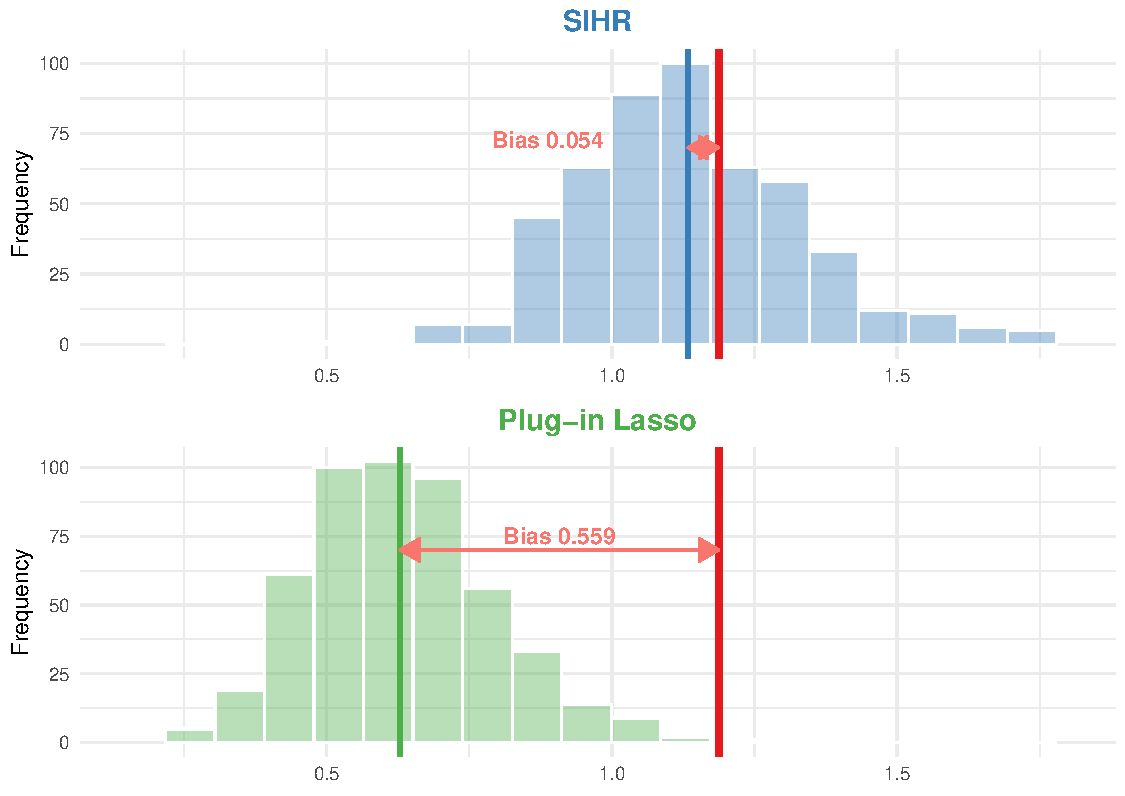
\includegraphics[width=0.7\linewidth]{SIHR-Bias.pdf}
    \caption{Comparison of the debiased estimates output by \CRANpkg{SIHR} and plug-in Lasso estimates for $\xnew^\intercal \beta$ in the logistic model with $n=400$. The upper panel shows the bias-corrected point estimates derived using our package \CRANpkg{SIHR}, while the lower panel features the plug-in point estimates from the \CRANpkg{glmnet} package. Red vertical lines indicate the target value $\xnew^\intercal \beta = 1.1875$. Biases between this target and the empirical means of the estimates are highlighted for each method.} %\Zhenyu{Prabrisha, please double check the setting is logistic and $n$}}
    \label{fig: bias plot}
\end{figure}

\subsection{Comparison with other inference methods}
We compare the performance of the \CRANpkg{SIHR} package with existing softwares, including R packages \CRANpkg{hdi} and \pkg{SSLasso}. The performance metrics include the empirical coverage, averaged length of confidence intervals, and averaged computational time (in seconds). All metrics are reported as the average of 500 simulation rounds. The confidence intervals based on \CRANpkg{hdi} and \pkg{SSLasso} are defined as follows:
\[
{\rm CI}_\alpha(\xnew) = \left(\xnew^\intercal \widetilde{\beta} - z_{\alpha/2} (\xnew^\intercal\widetilde{V}\xnew)^{1/2}, \quad
\xnew^\intercal\widetilde{\beta} + z_{\alpha/2} (\xnew^\intercal\widetilde{V}\xnew)^{1/2}
\right),
\]
%\Zijian{Zhenyu, check my expression.}
where $\widetilde{\beta}$ denotes the debiased estimator and $\widetilde{V}$ denotes the estimated covariate matrix of $\widetilde{\beta}$, outputted by \CRANpkg{hdi} and \pkg{SSLasso}.
Note that \pkg{SSLasso} only provides inference for linear regression models.
\vspace{-5mm}
\paragraph{Coverage and Length} As shown in Table \ref{tab: comparison}, the CIs based on \CRANpkg{SIHR} achieve desired coverage across various scenarios, and the lengths decrease with larger sample sizes. In contrast, the coverage of CIs from \CRANpkg{hdi} and \pkg{SSLasso} may be slightly undercovered, especially when $n=200$.
\vspace{-5mm}
\paragraph{Computation Efficiency}
We examine the computational efficiency of these methods and report the average computation time in the "Time" column, measured in seconds. The \CRANpkg{SIHR} package demonstrates notable computational efficiency, with an average processing time of under 10 seconds. In comparison, using the algorithm in \CRANpkg{hdi} with parameters $n=400$ and $p=300$ requires approximately 8 minutes. This significant difference stems from the fact that the \CRANpkg{hdi} algorithm is not tailored for inferring linear functionals and separately implementing $p$ bias correction steps, one for each regression coefficient, while \CRANpkg{SIHR} only implements a single bias correction step.

\begin{table}[!ht]
\centering
%\label{tab: Ex App}
\scalebox{0.75}{
\begin{tabular}{|r|r|rrr|rrr|}
%   \hline
% %  \hline
% \multicolumn{8}{|c|}{{\bf Linear Functional}} \\
  \hline
  \multicolumn{2}{|c|}{}&\multicolumn{3}{c|}{Linear}&\multicolumn{3}{c|}{Logistic} \\
   \hline
$n$ & Method & Cov & Len & Time & Cov & Len & Time \\
\hline
 \multirow{3}{*}{200} & \textbf{SIHR} & {0.94} & 0.47 & 3 & {0.94} & 0.94 & 3 \\ 
 & {hdi} & 0.90 & 0.38 & 211 & 0.91 & 0.80 & 213 \\
 & {SSLasso} & 0.83 & 0.34 & 17 & - & - & - \\
 \hline
 \multirow{3}{*}{400} & \textbf{SIHR} & {0.96} & 0.34 & 12 & {0.96} & 0.74 & 14 \\ 
 & {hdi} & 0.94 & 0.27 & 475 & 0.89 & 0.56 & 489 \\
 & {SSLasso} & 0.94 & 0.29 & 38 & - & - & - \\
 \hline
\end{tabular}
}
\caption{Comparison of methods implemented by packages \CRANpkg{SIHR}, \CRANpkg{hdi}, \pkg{SSLasso} in both linear and logistic models with $n\in \{200,400\}$. The columns labeled "Cov" and "Len" denote the empirical coverage and the length of the confidence intervals over 500 simulation runs, respectively; "Time" indicates the average computation time in seconds. The columns titled "Linear" and "Logistic" refer to the regression model applied. According to the experimental design, a valid inference method should achieve a coverage rate of approximately 0.95.%{\color{red}Shouldn't we separately mention what bolded coverage means?}
}
\label{tab: comparison}
\end{table}

%%%%%%%%%%%%%%%%%%%%%%%%%%%%%%%%%%%%%%%%%%%%%%%%%%%%%%%%%%%%%%%%%%%%%%%%%%%%%%%%%%%%%%%%%%%%%%%%%%%%%%%%%%%%%%%%%%%%%%%%%%%%%%%%%%%%%%%%%%%%%%%%%%%%%%

% \begin{itemize}
%     \item \textit{Plug-in} \CRANpkg{hdi}: The plug-in estimator $\xnew^\intercal \widehat{\beta}_{\rm hdi}$ is used to estimate $\xnew^\intercal \beta$, with the estimated variance $\widehat{V}_{\rm hdi}$, where $\widehat{\beta}_{\rm hdi}$ is the coordinate debiased Lasso estimator constructed by \CRANpkg{hdi}.
%     \item \textit{Plug-in} \pkg{SSLasso}: The plug-in estimator $\xnew^\intercal \widehat{\beta}_{\rm ss}$ is used to estimate $\xnew^\intercal \beta$, with the estimated variance $\widehat{V}_{\rm ss}$, where $\widehat{\beta}_{\rm ss}$ is the coordinate debiased Lasso estimator constructed by \pkg{SSLasso}. It is to be noted that \pkg{SSLasso} can produce inference only in the case of linear regression.
%     \item \textit{Post-selection Lasso}: Begin by identifying significant predictors using a penalized regression estimator denoted as $\widehat{\beta}$ in equation \eqref{eq: initial estimator}. Subsequently, apply a conventional low-dimensional (linear/logistic) regression model using the chosen predictors. The post-selection estimator, denoted as $\widehat{\beta}_{\rm PL}\in \mathbf{R}^{p}$, is then employed to estimate $\xnew^{\intercal}\beta$ as $\xnew^{\intercal}\widehat{\beta}_{\rm PL}$. The variance of this post-selection estimator, $\xnew^{\intercal}\widehat{\beta}_{\rm PL}$, can be computed using inference techniques from classical low-dimensional regression, represented as $\widehat{V}_{\rm PL}$.
    
%     \item \textit{Plug-in Lasso}: This estimator estimates $\xnew^{\intercal}\beta$ by $\xnew^{\intercal}\widehat{\beta}$ with $\widehat{\beta}$ denoting the penalized estimator in \eqref{eq: initial estimator}.
% \end{itemize}
% The inference procedures based on plug-in \CRANpkg{hdi}, \pkg{SSLasso} and post-selection Lasso are defined as
% \[
% {\rm CI}_\alpha(\xnew) = \left(\xnew^\intercal \widetilde{\beta} - z_{\alpha/2} \widetilde{V}^{1/2}, \quad
% \xnew^\intercal\widetilde{\beta} + z_{\alpha/2} \widetilde{V}^{1/2}
% \right),
% \]
% with replacing $(\widetilde{\beta}, \widetilde{V})$ by $(\widehat{\beta}_{\rm hdi}, \widehat{V}_{\rm hdi}), (\widehat{\beta}_{\rm ss}, \widehat{V}_{\rm ss})$ and $(\widehat{\beta}_{\rm PL}, \widehat{V}_{\rm PL})$ respectively.

% \noindent We vary sample size $n \in \{200,400\}$ and fix $p = 300$. The regression coefficient $\beta$ is generated as $\beta_1 = 0.5, \beta_2 = 0.75, \beta_3 = 0.25$ and $\beta_j = 0$ if $4 \leq j \leq p$. The intercept is set as $0$ since the R package \CRANpkg{hdi} excludes the intercept while performing the inference. The loading is set as $\xnew = (1, 0.75, 0.5, 0_{p-3})^\intercal$ so that $\xnew^{\intercal}\beta = 1.19$. 



%\begin{table}[!ht]
%\centering
%\scalebox{0.8}{
%\begin{tabular}{|r|r|rrr|rrr|}
%  \hline
%\multicolumn{8}{|c|}{{\bf Linear Functional}} \\
%  \hline
%  \multicolumn{2}{|c|}{}&\multicolumn{3}{c|}{Linear}&\multicolumn{3}{c|}{Logistic} \\
%   \hline
%$n$ & Method & Bias & SE & RMSE & Bias & SE & RMSE \\
%\hline
% \multirow{4}{*}{200} & SIHR & -0.05 & 0.11 & 0.12 & -0.11 & 0.26 & 0.29 \\ 
% & \texttt{hdi} & -0.01 & 0.11 & 0.11 & -0.12 & 0.21 & 0.24 \\
% & \pkg{SSLasso} & -0.11 & 0.09 & 0.15 & NA & NA & NA \\
% & Post-Selection & -0.09 & 0.12 & 0.14 & 8.59 & 46.95 & 47.73 \\
% & Plug-in Lasso & -0.34 & 0.12 & 0.35 & -0.74 & 0.23 & 0.77 \\
% \hline
% \multirow{4}{*}{400} & SIHR & -0.00 & 0.09 & 0.09 & -0.05 & 0.20 & 0.21 \\ 
% & \texttt{hdi} & 0.00 & 0.07 & 0.07 & -0.10 & 0.14 & 0.18 \\
% & \pkg{SSLasso} & 0.03 & 0.08 & 0.08 & NA & NA & NA \\
% & Post-Selection & -0.02 & 0.07 & 0.08 & 0.15 & 0.35 & 0.39 \\
% & Plug-in Lasso & -0.22 & 0.08 & 0.24 & -0.56 & 0.16 & 0.58 \\
% \hline
%\end{tabular}
%}
%\caption{The columns indexed with ``Bias",``SE" and ``RMSE" represent the empirical bias, standard error and root mean squared error respectively averaged over 500 rounds of simulations. The columns under "Linear" and "Logistic" correspond to the regression model considered. 
%}
%\label{tab: comparison estimation}
%\end{table}

%{\color{blue} We also report the bias, the standard deviation and Root Mean Squared Error (RMSE) of the proposed \CRANpkg{SIHR}, \CRANpkg{hdi}, \pkg{SSLasso}, post-selection and plug-in Lasso estimators in Table \ref{tab: comparison}. Plug-in Lasso estimator estimates $\xnew^{\intercal}\beta$ by $\xnew^{\intercal}\widehat{\beta}$ with $\widehat{\beta}$ denoting the penalized estimator in \eqref{eq: initial estimator}. The plug-in Lasso estimator is found unsuitable for constructing confidence intervals due to its bias component dominating its variance component. Upon comparing the proposed method with the plug-in Lasso estimator, it becomes evident that while the bias component diminishes, there is a corresponding rise in the variance. For enhanced visualization, we generate histograms representing the plug-in Lasso, post-selection, and \CRANpkg{SIHR} estimators for logistic regression with a sample size of $n = 400$ in Fig. \ref{fig: bias plot}. The analysis distinctly reveals that the \CRANpkg{SIHR} estimator exhibits the least bias, whereas the plug-in Lasso demonstrates the highest bias. In essence, the \CRANpkg{SIHR} method effectively mitigates the bias inherent in the conventional plug-in Lasso approach. %{\color{red} Moreover, across all scenarios, the estimators from the \CRANpkg{SIHR} package exhibit the smallest empirical bias, indicating the effectiveness of the bias correction approach.}}

% \begin{table}[!ht]
% \centering
% %\label{tab: Ex App}
% \scalebox{0.7}{
% \begin{tabular}{|r|r|rrrrrr|rrrrrr|}
%   \hline
% %  \hline
% \multicolumn{14}{|c|}{{\bf Linear Functional}} \\
%   \hline
%   \multicolumn{2}{|c|}{}&\multicolumn{6}{c|}{Linear}&\multicolumn{6}{c|}{Logistic} \\
%    \hline
% $n$ & Method & Cov & Len & Time & Bias & SE & RMSE & Cov & Len & Time & Bias & SE & RMSE \\
% \hline
%  \multirow{5}{*}{200} & \textbf{SIHR} & {0.94} & 0.47 & 3 & -0.05 & 0.11 & 0.12 & 0.94 & 0.94 & 3 & -0.11 & 0.26 & 0.29\\ 
%  & {hdi} & 0.88 & 0.38 & 217 & -0.01 & 0.11 & 0.11 & 0.89 & 0.80 & 209 & -0.12 & 0.21 & 0.24 \\
%  & {SSLasso} & 0.83 & 0.34 & 22 & -0.11 & 0.09 & 0.15 & - & - & - & - & - & - \\
%  & Post-Selection & 0.75 & 0.33 & 0.4 & -0.09 & 0.12 & 0.35 & 0.64 & 11763 & 2 & 8.59 & 46.95 & 47.73 \\
%  & Plug-in & - & - & 0.7 & -0.34 & 0.12 & 0.35 & - & - & 2 & -0.74 & 0.23 & 0.77 \\
%  \hline
%  \multirow{5}{*}{400} & \textbf{SIHR} & {0.96} & 0.34 & 12 & -0.00 & 0.09 & 0.09 & 0.96 & 0.74 & 15 & -0.05 & 0.20 & 0.21 \\ 
%  & {hdi} & 0.93 & 0.27 & 459 & 0.00 & 0.07 & 0.07 & 0.89 & 0.56 & 493 & -0.10 & 0.14 & 0.18 \\
%  & {SSLasso} & 0.94 & 0.29 & 38 & 0.03 & 0.08 & 0.08 & - & - & - & - & - & - \\
%  & Post-Selection & 0.90 & 0.25 & 1 & -0.02 & 0.07 & 0.08 & 0.80 & 0.75 & 3 & 0.15 & 0.35 & 0.39 \\
%  & Plug-in & - & - & 2 & -0.22 & 0.08 & 0.24 & - & - & 4 & -0.56 & 0.16 & 0.58 \\
%  \hline
% \end{tabular}
% }
% \caption{The columns indexed with "Cov" and "Len" represent the empirical coverage and length of the CIs in 500 rounds of simulations; "Time" represents the averaged computation time (in seconds) while the columns indexed with "Bias",`"SE" and "RMSE" represent the empirical bias, standard error and root mean squared error respectively averaged over 500 rounds of simulations. The columns under "Linear" and "Logistic" correspond to the regression model considered. {\color{red} Do we need to bold the ones where there is coverage?}
% }
% \label{tab: comparison}
% \end{table}



% \begin{center}
%     \begin{figure}
%         \centering
%         \includegraphics[scale = 0.45]{Bias_Plot_xaxis.jpeg}
%         \caption{Histogram of point estimates using \code{SIHR}, plug-in LASSO and post selection LASSO.}
%         \label{fig: bias plot same x}
%     \end{figure}
% \end{center}

\section{Real data applications}
\label{sec: real data}

\subsection{Motif regression}
We showcase the application of the \code{LF()} function in motif regression analysis, which investigates the impact of motif matching scores on gene expression levels, as discussed in the literature \citep{beer2004predicting, conlon2003integrating, das2004interacting, yuan2007predicting}. Motifs are specific DNA sequences bound to transcription factors, playing crucial roles in controlling transcription activities, such as gene expressions \citep{yuan2007predicting}. The matching score of a motif measures its prevalence, reflecting how prominently a motif appears in the upstream regions of genes. These matching scores are recognized for their effectiveness in predicting gene expression levels. Our goal is to quantitatively assess the association between these matching scores and gene expression, elucidating the underlying biological mechanisms. In this analysis, we work with a dataset that includes the expression levels of $n=2587$ genes, where matching scores of $p=666$ motifs are observed on each gene. The structure of the data is organized as follows: for $1\leq i\leq 2587$,
\begin{itemize}
    \item $y_i: \textrm{the expression level of gene $i$};$
    \item $X_{i,j}: \textrm{the matching score of the $j$-th motif on gene $i$, for $1\leq j\leq 666$.}$
\end{itemize}

% $$
% \begin{aligned}
% y_i : & \text{the expression level of gene $i$}; \\
% X_{i,j} : & \textrm{the matching score of the $j$-th motif on gene $i$, for $1\leq j\leq 666$.} 
% \end{aligned}
% $$
Below, we display several observations of the response variable along with the first four covariates out of a total of 666.
\begin{example}
    colnames(X) <- paste0("X",1:ncol(X))
    head(cbind(y, X[,1:4]))
    #>               y        X1       X2       X3       X4
    #>   YAL002W  0.51 1.1595129 1.573024 1.239862 1.144537
    #>   YAL003W -3.06 1.9581497 1.928997 1.228753 1.118513
    #>   YAL007C -1.86 1.3047351 1.617691 1.299527 1.126370
    #>   YAL025C -1.54 0.8057353 1.487356 1.395147 1.003005
    #>   YAL034C  1.00 0.8886961 1.860788 1.569881 1.316531
    #>   YAL035W -2.05 1.3377646 1.152577 1.532653 1.012072
\end{example}

% We provide summary statistics for the response variable and the first four covariates out of 666, which offers a preliminary insight into the dataset's composition. 
% \begin{example}
%     colnames(X) <- paste0("X",1:ncol(X))
%     data <- cbind(y, X[,1:4])
%     summary(data)
%     #>       Y               X1               X2              X3              X4
%     #>   Min.   :-6.640   Min.   :0.000   Min.   :0.000   Min.   :0.000   Min.   :0.000
%     #>   1st Qu.:-1.940   1st Qu.:0.857   1st Qu.:1.258   1st Qu.:1.220   1st Qu.:1.072
%     #>   Median :-0.670   Median :1.127   Median :1.398   Median :1.340   Median :1.189
%     #>   Mean   :-0.410   Mean   :1.231   Mean   :1.430   Mean   :1.360   Mean   :1.209
%     #>   3rd Qu.: 1.045   3rd Qu.:1.393   3rd Qu.:1.568   3rd Qu.:1.483   3rd Qu.:1.323
%     #>   Max.   : 7.150   Max.   :2.669   Max.   :2.748   Max.   :2.330   Max.   :2.697
% \end{example}

\noindent 
We seek to investigate the relationships between the matching scores of individual motifs ($X_{\cdot,j}$ for $1 \leq j \leq 666$) and gene expression levels ($y$). Our objective is to access the significance of these associations. For this purpose, the \code{LF()} function from the package \CRANpkg{SIHR} is utilized to compute 95\% confidence intervals for the 666 regression coefficients.
\begin{example}
    p <- ncol(X)
    loading.mat <- diag(p)
    Est <- LF(X, y, loading.mat, model='linear')
    ci(Est)
\end{example}
We then summarize and visualize the resulting 666 confidence intervals in Figure \ref{fig: t134}.
The results reveal that 25 of these intervals, highlighted in {\color{NeonBlue} blue}, lie entirely above zero, indicating a positive association between the matching scores of these specific motifs and gene expression levels. Conversely, 23 intervals, marked in {\color{NeonGreen} green}, fall completely below zero, suggesting a negative influence of these motifs on gene expression levels. Overall, these results demonstrate that 48 motifs out of the total have a statistically significant influence on gene expression, offering valuable insights into the regulatory mechanisms involved.
%{\color{red}Code for figure?}

\begin{figure}[!ht]
\centering
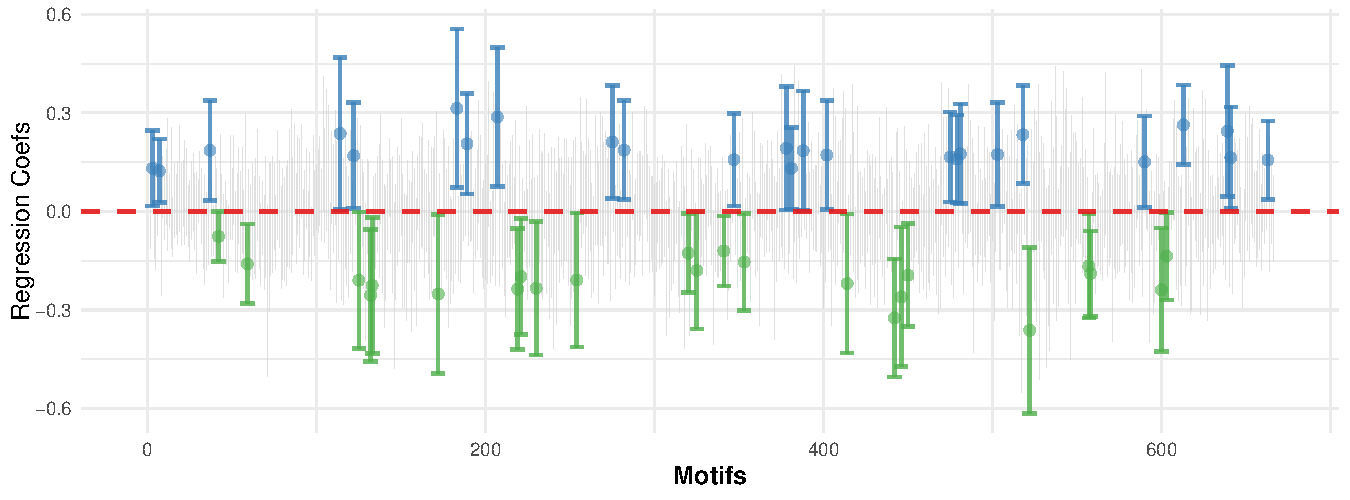
\includegraphics[width = 0.9\textwidth]{CI-Motif.pdf}
\caption{Motif: Constructed CIs for the 666 regression coefficients. Motifs represented by {\color{NeonBlue} blue} CIs indicate a significant positive association with gene expression levels, whereas those with {\color{NeonGreen} green} CIs demonstrate significant negative associations.} 
\label{fig: t134}
\end{figure}

\subsection{Fasting glucose level data}
We have illustrated the application of the \code{LF()} function in a linear regression context. We now demonstrate its use on another real application in a logistic regression setting. In this study, we examine the impact of polymorphic genetic markers on glucose levels in a stock mice population. The data, accessible at \url{https://wp.cs.ucl.ac.uk/outbredmice/heterogeneous-stock-mice/}, uses fasting glucose levels, dichotomized at $11.1$ mmol/L, as the response variable —an important indicator for type-2 diabetes. Specifically, glucose levels below $11.1$ mmol/L are considered normal and labeled as $y_i = 0$, while levels above $11.1$ mmol/L are classified as high, indicating pre-diabetic or diabetic conditions, and labeled as $y_i=1$.

The dataset initially comprises $10,346$ polymorphic genetic markers for a sample size $n=1,269$. Given the large number of markers and the significant correlation among some of them, we implement a selection criterion to ensure the maximum absolute correlation among the markers does not exceed $0.75$. After filtering, we narrow down to a subset of $2, 341$ genetic markers. Additionally, we include "gender" and "age" as baseline covariates. To prepare for the analysis, both the genetic markers and baseline covariates are standardized.
To sum up, the data structure is organized as follows: for $i = 1,\ldots,1269$:
\begin{itemize}
    \item $y_i: \textrm{ binary indicator of whether the fasting glucose level is above $11.1$ mmol/L}$
    \item $X_{i,j}: \textrm{ genetic marker $j$ for mouse $i$ with $j=1,\ldots,2341$}$
    \item $X_{i, 2342}: \textrm{ gender of mouse $i$}$
    \item $X_{i,2343}: \textrm{ age of mouse $i$}$
\end{itemize}
\noindent Below, we display several observations of the response variable along with the first four covariates out of a total of 2343.
\newpage
\begin{example}
    head(cbind(y, X[,1:4]))
    #>              y rs3674785_G rs13475705_A rs13475706_G rs3684358_C
    #>   A048005080 1    0.184158   -0.5697056    0.6063887  -0.3444252
    #>   A048006555 0   -1.258413   -0.5697056   -0.9113771   1.1272098
    #>   A048007096 0    0.184158    1.5137423   -0.9113771  -0.3444252
    #>   A048010273 1   -1.258413   -0.5697056   -0.9113771   1.1272098
    #>   A048010371 0    0.184158   -0.5697056    0.6063887  -0.3444252
    #>   A048011287 0    0.184158    1.5137423   -0.9113771  -0.3444252
\end{example}


\noindent Given the real dataset, we aim to investigate the association of each polymorphic marker ($X_{\cdot, j}$ for $1\leq j\leq 2341$) with fasting glucose levels ($y$) and determine the statistical significance of each association. We employ the function \code{LF()} configured with \code{model = "logistic"} to compute confidence intervals for the initial 2341 regression coefficients, which correspond to all polymorphic markers, as demonstrated in the following code:
\begin{example}
    p <- ncol(X)
    loading.mat <- diag(p)[,-c(2342,2343)]
    Est <- LF(X, y, loading.mat, model='logistic')
    ci(Est)
\end{example}
We then visualize the obtained 2341 confidence intervals in Figure \ref{fig: logistic CI}.
It reveals that 13 genetic markers display CIs exclusively above $0$ (marked in {\color{NeonBlue}blue}), signifying a significant positive correlation with fasting glucose levels. Conversely, 16 markers exhibit CIs entirely below $0$ (marked in {\color{NeonGreen} green}), denoting a significant negative correlation with fasting glucose levels. These results showcase that 29 genetic markers out of the total have a statistically significant impact on glucose levels.

\begin{figure}[!ht]
\centering
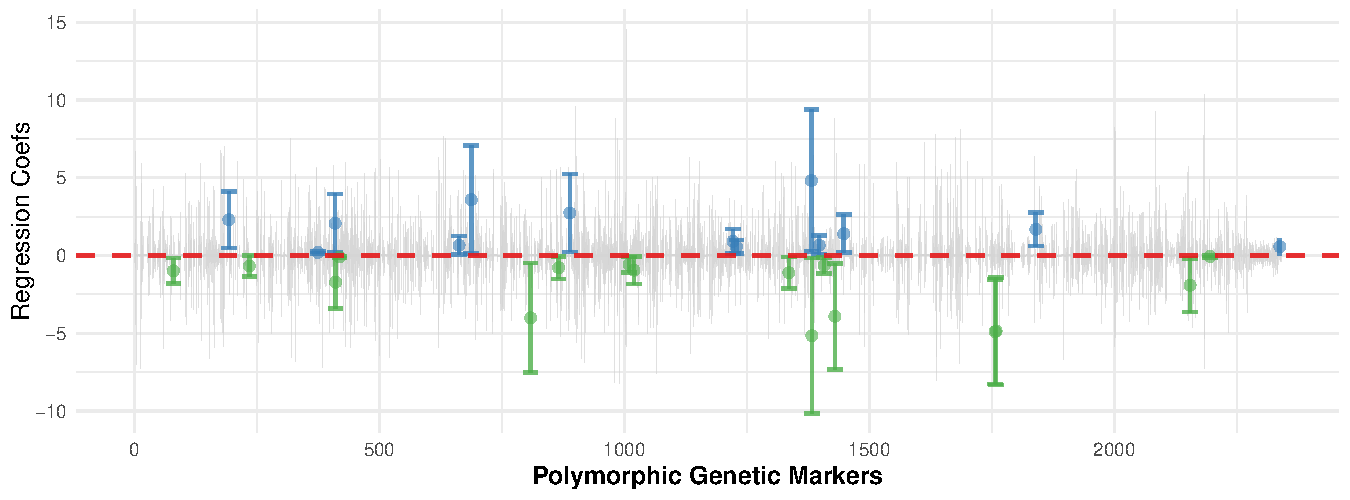
\includegraphics[width = 0.9\textwidth]{CI-Glucose.pdf}
\caption{Glucose: Constructed CIs for the first $2341$ regression coefficients. Genetic markers represented by {\color{NeonBlue} blue} CIs indicate a significant positive association with the fasting glucose level, whereas those with {\color{NeonGreen} green} CIs demonstrate significant negative associations.} 
\label{fig: logistic CI}
\end{figure}

\section{Conclusion}

There has been significant recent progress in debiasing inference methods for high-dimensional GLMs. This paper highlights the application of advanced debiasing techniques in high-dimensional GLMs using the R package \CRANpkg{SIHR}. The package provides tools for estimating bias-corrected point estimators and constructing CIs for various low-dimensional objectives in both one- and two-sample regression settings. Through extensive simulations and real-data analyses, we demonstrate the practicality and versatility of the package across diverse fields of study, making it an essential addition to the literature.

\section{Acknowledgement}
Prabrisha Rakshit and Zhenyu Wang contributed equally to this work and are considered co-first authors. Dr. Tony Cai’s research was supported in part by NSF grant DMS-2015259 and NIH grants R01-GM129781 and R01-GM123056. Dr. Zijian Guo’s research was supported in part by NSF grants DMS-1811857 and DMS-2015373 and NIH grants R01-GM140463 and R01-LM013614. Dr. Zijian Guo is grateful to Dr. Lukas Meier for sharing the motif regression data used in this paper.

\bibliography{rakshit-wang}


\address{Prabrisha Rakshit\\
  Rutgers, The State University of New Jersey\\
  USA\\
  \email{prabrisha.rakshit@rutgers.edu}}

\address{Zhenyu Wang\\
  Rutgers, The State University of New Jersey\\
  USA\\
  \email{zw425@stat.rutgers.edu}}

\address{Tony Cai\\
  University of Pennsylvania\\
  USA\\
  \email{tcai@wharton.upenn.edu}}
  
\address{Zijian Guo\\
  Rutgers, The State University of New Jersey\\
  USA\\
  \email{zijguo@stat.rutgers.edu}}  

